\documentclass[12pt,oneside,final]{book}
\usepackage[portuges,brazil]{babel}
%\usepackage[latin1]{inputenc}

%=============================================
% Define fonte arial:
%\usepackage[scaled]{uarial}
%\renewcommand*\familydefault{\sfdefault}
%=============================================
% Na linha abaixo, coloque os pacotes que você usa.
% Quanto menos pacotes você colocar, mais rápida será
% a compilação de seu texto
\usepackage{icomma,indentfirst,ae,amssymb,
fancyhdr,fancybox,epsfig,psfrag,amsmath,
tabularx,url}
\usepackage{comment}


% Este pacote define o tamanho do papel (página) e as margens
\usepackage[a4paper,hmargin={25mm,20mm},vmargin={20mm,20mm}]{geometry}

% Este pacote usa parênteses no lugar de colchetes nas citações
\usepackage[round]{natbib}


\usepackage[color]{showkeys}
\definecolor{refkey}{rgb}{0.39,0.58,1}
\definecolor{labeled}{rgb}{1,0,0}
\usepackage[Lenny]{fncychap}
\setlength{\headheight}{15pt}
\usepackage{hyperref}
\usepackage[all]{hypcap}

%===================== Cabecalhos =====================

\renewcommand{\chaptermark}[1]{\markboth{\chaptername\ \thechapter. \ #1}{ }}
\renewcommand{\sectionmark}[1]{\markright{\thesection. \ #1}}

%\lhead{\nouppercase{\leftmark}}
\lhead{}
%\chead{}
\rhead{\nouppercase{\rightmark}}
%\lfoot{From: K. Grant}
\cfoot{\thepage}
%\rfoot{\thepage}
%==============================================================================================

%===========================
%  Coloque aqui os novos comandos que vc definir

%================================
% Comandos já definidos (vale a pena dar uma olhada geral)

% Espacos H2, Hoo, L2, Loo
\newcommand\Hi{{\mathcal{H}}_{\infty}}
\newcommand\Hd{{\mathcal{H}}_{2}}
\newcommand\Li{{\mathcal{L}}_{\infty}}
\newcommand\Ld{{\mathcal{L}}_{2}}


\def\reais{{\rm I\kern-.17em R}} % R de reais
\def\Dest{{\rm I\kern-.17em D}} % R de reais
\newcommand{\Dgest}{\ensuremath{\mathcal{D}}}
\newcommand{\naturais}{\mathbb{N}}
\newcommand{\inteiros}{\mathbb{Z}_{+}}
\newcommand{\matlab}{{\sc Matlab}}

%super parenteses
\makeatletter
\def\Biggg#1{{\hbox{$\left#1\vbox to29\p@{}\right.\n@space$}}}
\newdimen\bracketwidth
\settowidth{\bracketwidth}{\Biggg(} \makeatother


\newcommand{\carinha}{\raisebox{-.2ex}{\epsfxsize 3mm \epsffile{cara.eps}}}

% Bolds
\newcommand{\I}{{\bf I}}
\newcommand{\Z}{{\bf 0}}
\newcommand{\Bfres}{\mathcal{B}}

% funcoes
\newcommand{\Tr}{\mbox{Tr}}

% Referencia com parenteses
\newcommand{\bref}[1]{\mbox{(\ref{#1})}}

% Ambiente de equacoes
\newcommand\be{\begin{equation}}
\newcommand\ee{\end{equation}}
\newcommand\vi{\vspace{\baselineskip}}

% newtheorems e similares

\newtheorem{teorema}{\noindent{\bf Teorema} }[chapter]
\newtheorem{lema}{\noindent{\bf Lema} }[chapter]
\newtheorem{corolario}{\noindent{\bf Corolário} }[chapter]
\newenvironment{prova}{\noindent{\bf Prova:}}{\null\hfill $\rule{1.5mm}{1.5mm}$}
\newtheorem{definicao}{\noindent{\bf Definição} }[chapter]

\newcommand{\simplex}{\Delta_N}



\newcommand{\Aal}{A(\alpha)}
\newcommand{\Bal}{B(\alpha)}
\newcommand{\Cal}{C(\alpha)}
\newcommand{\Dal}{D(\alpha)}


\newcommand{\Pal}{P(\alpha)}
\newcommand{\Gal}{G(\alpha)}
\newcommand{\Hal}{H(\alpha)}
\newcommand{\Qal}{Q(\alpha)}
\newcommand{\Xal}{X(\alpha)}
\newcommand{\Xual}{X_1(\alpha)}
\newcommand{\Xdal}{X_2(\alpha)}

\newcommand{\Sfr}{\mathcal{S}}

\newcommand{\Xfal}{\mathcal{X}(\alpha)}
\newcommand{\Bfal}{\mathcal{B}(\alpha)}
\newcommand{\Qfal}{\mathcal{Q}(\alpha)}
\newcommand{\Sfal}{\mathcal{S}(\alpha)}

\newcommand{\Kfr}{\mathcal{K}}
\newcommand{\Ifr}{\mathcal{I}}
\newcommand{\Afr}{\mathcal{A}}
\newcommand{\Pfr}{\mathcal{P}}
\newcommand{\Cfr}{\mathcal{C}}
\newcommand{\Gfr}{\mathcal{G}}

% Colchetes e parênteses maiores
\newcommand{\PR}[1]{\ensuremath{\left[#1\right]}}
\newcommand{\PC}[1]{\ensuremath{\left(#1\right)}}

\newcolumntype{L}{>$l<$}

% Tabelas Preenchidas
\usepackage{booktabs}
\usepackage[table,xcdraw]{xcolor}

\usepackage{subfigure}

\usepackage{minted}

\usepackage{float} % Arquivo com todas as macros

%============================================
% Defina seus dados:
%============================================
\newcommand\autor{Matheus Ferreira Costa}
\newcommand\titulo{Construção e controle de um sistema do tipo pêndulo invertido \\ sobre duas Rodas}
\newcommand\orientador{Prof. Dr. Luís Filipe Pereira Silva}
%\newcommand\coorientador{Prof. Dr. Juliano de Barros Veloso e Lima}
\newcommand\cidade{Divinópolis, MG}
\newcommand\ano{$2022$}
%============================================


\begin{document}

%\usepackage{comment}

%========= Paginas iniciais ==============
% Muda numeração para usar algarismos romanos
\pagenumbering{roman}
\pagestyle{fancy}
%=================================================
% Use o comando abaixo para TCC II
    %================================================================================================
%=========================================== CAPA 1 =============================================
%================================================================================================
\vspace*{1.0cm}

\begin{center}
{\sc  Centro Federal de Educação Tecnológica de Minas Gerais\\ {\em Campus} Divinópolis\\ Graduação em Engenharia Mecatrônica}
\end{center}

\vspace*{3.0cm}

\begin{center}
\large \autor % alterar também mais abaixo.
\end{center}


\vspace*{2.5cm}

\begin{center}
{\sc  \titulo} % alterar também mais abaixo.
\end{center}

\vspace*{4cm}

\epsfxsize=0.175\columnwidth
\centerline{\epsffile{logocefet}}

\null\vfill

\begin{center}
\cidade\\\ano % alterar também mais abaixo.
\end{center}


%Não numera a página:
\thispagestyle{empty}

%================================================================================================
%=========================================== CAPA 2 =============================================
%================================================================================================
\newpage
\vspace*{1.2cm}

\begin{center}
\large \autor % alterar também mais acima.
\end{center}


\vspace*{3.0cm}

\begin{center}
{\sc \titulo}  % alterar também mais acima.
\end{center}

\vspace*{2.5cm}

\begin{flushright}
\begin{minipage}{9.0cm}
Monografia de Trabalho de Conclusão de Curso apresentada ao
Colegiado de Graduação em Engenharia Mecatrônica
como  parte dos requisitos exigidos para a obtenção do título de
Engenheiro Mecatrônico.  \\
Áreas de integração: {Controle e Mecânica}.

\vspace*{1cm}

Orientador: \orientador \\
%Co-orientador: \coorientador
\end{minipage}
\end{flushright}

\vspace*{2.5cm}

%\epsfxsize=0.175\columnwidth
%\centerline{\epsffile{logocefet}} % Aqui poderia ser substituido por um logo do curso ou do campus

\null\vfill

\begin{center}
\cidade\\\ano  % alterar também mais acima.
\end{center}


%Não numera a página:
\thispagestyle{empty}

%================================================================================================
%=========================================== CAPA 3 =============================================
%================================================================================================
\newpage

\vspace*{1.2cm}
\begin{center}
\large \autor\\%[-1mm] % se for preciso ajustar a altura do texto
\end{center}


\vspace*{1.8cm}

\begin{center}
{\sc  \titulo}
\end{center}

\vspace*{2.25cm}

\begin{flushright}
\begin{minipage}{9.0cm}
Monografia de Trabalho de Conclusão de Curso apresentada ao
Colegiado de Graduação em Engenharia Mecatrônica
como  parte dos requisitos exigidos para a obtenção do título de
Engenheiro Mecatrônico.  \\
Áreas de integração: {Controle e Mecânica}.\\


\vspace*{0.5cm}

\end{minipage}
\end{flushright}

\vspace*{2cm}

\noindent Comissão Avaliadora:
\vspace*{0.5cm}

\noindent \begin{minipage}{0.5\linewidth}
Prof. Dr. Luís Filipe Pereira Silva \\[1mm]
CEFET/MG {\em Campus} Divinópolis
\end{minipage}
\begin{minipage}{0.5\linewidth}
Prof. Dr. Jean Carlos Pereira \\[1mm]
CEFET/MG {\em Campus} Divinópolis
\end{minipage}

\vspace*{0.4cm}

\noindent \begin{minipage}{0.5\linewidth}
\noindent  Prof. Dr. Lucas Silva de Oliveira \\[1mm]
\noindent  CEFET/MG {\em Campus} Divinópolis
\end{minipage}

\null \vfill

\begin{center}
\cidade\\\ano
\end{center}

%Não numera a página:
\thispagestyle{empty}
%======================================== Dedicatória =========================================
\newpage
\chapter*{}
\null
\vfill
\begin{flushright}
\begin{minipage}{6.5cm}
{\sc Ao meu pai.}
\end{minipage} \\[8mm]
\end{flushright}

%==============================================================================================

%======================================= Agradecimentos =======================================
\newpage
\chapter*{Agradecimentos}


\noindent Agradeço,\\[2mm]
\begin{itemize}
    \item aos meus avós João Custódio (vô Ló) e Maria das Dores (vó Lia), que sempre cuidaram de mim, da minha mãe e meus irmãos quando mais precisamos. Além de tudo, agradeço por me apoiarem e terem feito eu seguir o caminho dos estudos.
    \item à minha mãe Cintia Aparecida e meu padrasto Roni, por sempre me  apoiarem, ajudarem e serem os exemplos ao qual me espelho. Eu amo vocês incondicionalmente.
    \item à minha namorada Ruanna, pelo companheirismo inigualável e por sempre acreditar em mim e me fazer acreditar que sou capaz o tempo todo. Com você eu tenho certeza e clareza dos meus objetivos. Obrigado por aguentar todos esses anos de estudos ao meu lado e sempre me apoiar nesse meu sonho, amo você.
    \item ao Professor Dr. Luís Filipe Pereira Silva, pelo suporte, orientação e pelo compartilhamento de conhecimento para este trabalho e outros para a vida como a ``bastter.com".
    \item ao professor Dr. Jean Carlos Pereira, que me identifiquei bastante e pude trabalhar em projetos de pesquisa ao longo do curso, inclusive este que antes de se tornar um trabalho final de curso foi tema de pesquisa.
    \item aos meus irmãos Ana Paula e Yuri, que são tudo para mim. Eu, por ser o mais velho, tenho o sentimento de sempre cuidar de vocês, então é isso que sempre tento fazer. E por mais que temos nossas brigas de irmãos, sou muito sortudo por ter vocês em minha vida.
    \item à turma 8, por todos os ``burgões", pelos momentos de descontração e pelas amizades que levarei para sempre no coração. Vocês tornaram a caminhada mais leve e divertida.
    \item ao meu companheiro Delgado, principalmente, durante este trabalho. Foram algumas reuniões bem longas após o fim de trabalho e você sempre se prontificou a me ajudar.
    \item ao meu amigo de longa data Mateus Pereira, em especial, por ter emprestado sua fresa e seu galpão mecânico para construção da estrutura física da planta.
    \item aos meus colegas de turma, Duda, Maria Vitória e Kesley, que hoje está se tornando uma grande amizade. Obrigado por confiarem que eu seria capaz, me apoiarem e até por emprestarem uma ponte H aos 45 do segundo tempo.
    \item ao corpo docente e funcionário do CEFET-MG \textit{Campus} Divinópolis, pela colaboração e atenção.

\end{itemize}

\vfill
%==============================================================================================
%======================================== Frase Miss Brasil ===================================
\newpage
\chapter*{}
\null\vfill
\begin{flushright}
\begin{minipage}{9.0cm}
Que todos os nossos esforços estejam sempre focados no desafio à impossibilidade. Todas as grandes conquistas humanas vieram daquilo que parecia impossível.
\end{minipage}
\end{flushright}


\begin{flushright}
 \href{https://viacarreira.com/epigrafe-para-tcc/}{Charles Chaplin}
\end{flushright}

%==============================================================================================


%=================================================

% Resumo e abstract (abstract somente para TCC II)
    %================================= Resumo e Abstract ========================================
\newpage

\chapter*{Resumo}

\vspace*{0.5cm}

\begin{quotation}
\noindent 
O sistema robotizado de pêndulo invertido se tornou largamente conhecido através do Segway nas últimas décadas, inspirando diversas pesquisas por sistemas de controle eficazes e robustos. Paralelamente, a versão autônoma do veículo também tem atraído a atenção da comunidade acadêmica por se tratar de um sistema não linear e instável em malha aberta. Dessa maneira, este trabalho teve por objetivo a construção e o controle de um sistema do tipo pêndulo invertido sobre duas rodas. Para isso, foram necessário vários estudos a respeito de controladores que consigam trabalhar em sistemas não lineares. Uma das técnicas de controle amplamente utilizadas em sistemas não lineares e com múltiplos estados é o LQG, que advém da teoria do controle ótimo. Este controlador, diferente de muitos que há na literatura, é bastante robusto o que faz com que o mesmo lide bem com ruídos e distúrbios. Após análise e desenvolvimento do projeto CAD, realizou-se a construção física da planta. De forma a simplificar os cálculos, descartou parâmetros como fricção e ruídos da modelagem matemática. As técnicas utilizadas na modelagem nos fornece inicialmente um modelo não linear contínuo no tempo, sendo necessário a realização da linearização utilizando equações Jacobianas e obtendo assim o espaço de estados do sistema. Como a placa que comandará a planta é um microcontrolador, realizou-se a discretização do sistema. Após isso, obteve-se o vetor de ganhos ótimos do LQR e do estimador. As primeiras validações se deu em ambiente simulado aplicando os ganhos do controlador na equação não linear contínua obtida na etapa da modelagem. Com mais essa etapa finalizada, realizou-se testes. Primeiramente, foi desenvolvido um código no Arduino em conjunto com Processing e VS Code, sendo possível validar os sinais do sensor e os motores. Após as validações, desenvolveu-se um código completo no Arduino para controle da planta.
\vspace*{0.5cm}

\noindent Palavras-chave: Segway. Pêndulo Invertido Sobre Duas Rodas. Controle Ótimo. Microcontrolador. LQG.

\end{quotation}



%===================================================================
% A parte abaixo não deve estar presente em TCC I, somente em TCC II.
%===================================================================
 \newpage

 \chapter*{Abstract}

 \vspace*{0.5cm}

 \begin{quotation}


 \noindent The inverted pendulum robotic system has become widely known through the Segway in recent decades, inspiring several researches for effective and robust control systems. At the same time, the autonomous version of the vehicle has also attracted the attention of the academic community because it is a non-linear and unstable open-loop system. Thus, this work aimed to build and control an inverted pendulum-type system on two wheels. For this, several studies were needed about controllers that can work in non-linear systems. One of the control techniques widely used in nonlinear and multi-state systems is LQG, which comes from the theory of optimal control. This controller, unlike many in the literature, is quite robust, which makes it handle noise and disturbances well. After analysis and development of the CAD project, the physical construction of the plant was carried out. In order to simplify the calculations, parameters such as friction and noise were excluded from the mathematical modeling. The techniques used in the modeling initially provide us with a nonlinear model continuous in time, being necessary to carry out the linearization using Jacobian equations and thus obtaining the state space of the system. As the board that will control the plant is a microcontroller, the system was discretized. After that, the vector of optimal gains of the LQR and the estimator was obtained. The first validations took place in a simulated environment by applying the controller gains in the continuous nonlinear equation obtained in the modeling stage. With this step completed, tests were carried out. First, a code was developed in Arduino together with Processing and VS Code, being possible to validate the sensor signals and the motors. After the validations, a complete code was developed in Arduino to control the plant.
 \vspace*{0.5cm}

 \noindent Key-words: Segway. Two-Wheeled Inverted Pendulum. Microcontroller. Optimal Control. LQG.
 \newpage% verso em branco
 \end{quotation}
%
%===================================================================


\tableofcontents

%========= lista de tabelas e figuras ==============

\listoffigures
    \addcontentsline{toc}{chapter}{Lista de Figuras}


\listoftables
    \addcontentsline{toc}{chapter}{Lista de Tabelas}


%============================Acronimos e Notação =================================================
\newpage

\chapter*{Lista de Acrônimos e Notação}
\addcontentsline{toc}{chapter}{Lista de Acrônimos e Notação}

\begin{tabular}{ll}
LQR  & Linear Quadratic Regulator (regulador linear quadrático)\\
LQE  & Linear Quadratic Estimator (estimador linear quadrático)\\
LQG  & Linear Quadratic Gaussian (linear gaussiano quadrático)\\
LTI  & Linear Time-Invariant (linear invariante no tempo)
\end{tabular}

\vspace*{1cm}

\begin{tabular}{ll}
$A$ & notação para matrizes (letras maiúsculas do alfabeto latino)\\
$\in$ & símbolo ``contido em''\\
$\forall$ & quantificação universal (``para todos; para qualquer; para cada'')\\
$\reais$ & conjunto dos números reais\\
$\mathbb{E}$ & símbolo para expectância ou esperança de uma variável aleatória\\
$\I$ & matriz identidade de dimensão apropriada\\
$n$ & especialmente utilizada para representar a ordem uma matriz quadrada\\
$\int$ & símbolo de integral\\
$\sum$ & notação de somatório\\
$\alpha$ & símbolos utilizados para simplificar os termos do modelo (letras gregas)
\end{tabular}


%==============================================================================================
 % arquivo com *todas* as notacoes e acronimos usados
    

%=================================================
\newpage


%\thispagestyle{empty}

% Muda espaçamento para 1,3 vezes maior que o padrão
\baselineskip 1.3\baselineskip

% Muda numeração para usar algarismos arábicos
\pagenumbering{arabic}
\pagestyle{fancy}
% Carrega os capítulos
\chapter{Introdução}\label{cap:Intro}

Neste capítulo introdutório tem como finalidade a apresentação do tema, os objetivos do trabalho realizado e relata-se a sequência em que foi desenvolvido. Primeiramente, a situação problema será apresentada. Em seguida, as principais motivações e objetivos propostos neste trabalho. Após esses pontos e para finalizar, a estrutura dos capítulos dessa dissertação será apresentada.

\section{Definição do Problema}

A realização do controle do pêndulo invertido, seja qual for sua variação, é um dos exemplos mais importantes na teoria de controle moderno. Sua estrutura resulta em um sistema não linear bastante complexo. Isso dificulta bastante a utilização de técnicas clássicas de teoria de controle.

O controle de sistemas não linear é uma técnica na qual um procedimento ou processo é conseguido sem a interferência humana. Para realizar a mesma, é preciso que um programa de instruções seja escrito  combinado a um sistema de controle que executa as tarefas. De acordo com \cite{Groover:11}, um processo automatizado necessita de energia não só para operar a condução do processo como para operar o programa e o sistema de controle. Ademais, considera-se uma grande aliada da otimização do desempenho, já que com essa tecnologia é possível conhecer indicadores que auxiliam a gestão, acelera os processos e remove trabalhos repetitivos, dispensáveis e não aceitáveis ergonomicamente.

Uma grande área em ascensão da robótica é a robótica móvel. Sendo assim, os robôs se locomovem dentro de um ambiente qualquer de diversas formas, com rodas, esteiras, pernas mecânicas, dentre outras. Estes robôs são caracterizados pela capacidade de se deslocar, podendo ser de modo guiado, semiautônomo ou totalmente autônomo \citep{Jung:05}. Algumas de suas mais variadas aplicações são: aspiração de pó, entrega de alimentos, vigilância predial, busca e salvamento, etc.

Assim sendo, neste trabalho, realizou-se o desenvolvimento de um veículo do tipo pêndulo invertido sobre duas rodas, que pode ser classificado como um robô do tipo móvel. Para a estabilização na vertical deste sistema, utilizou-se de técnicas de controle robustas que irão conseguir tratar as simplificações e considerações de seu modelo matemático. 

\section{Motivação}
O estudo da Teoria de Controle em sistemas dinâmicos e a implementação de controladores em uma planta física, complexa e com características não lineares, além da concretização de um projeto completo é de suma importância na consolidação dos conceitos assimilados ao longo da formação acadêmica de um profissional da área de Mecatrônica.

Além de tudo, após o estudo de três disciplinas seguidas da área de controle e a vontade do autor de conseguir realizar o controle de uma planta clássica, porém com um nível de dificuldade elevada bem como a construção de um projeto puramente mecatrônico que aborda as quatro grandes áreas: mecânica, controle, computação e eletrônica.

\section{Objetivos do Trabalho}
Aqui é descrito de forma sucinta o objetivo geral e os objetivos específicos do trabalho. Fazendo-se cumprir esses objetivos específicos, espera-se alcançar o objetivo geral.

\subsection{Objetivo Geral}
Construir um sistema denominado pêndulo invertido sobre duas rodas e controlar a posição de sua estrutura para que a mesma fique paralela com a vertical (0$^\circ$ ou 0 radianos) utilizando controlador ótimo.

\subsection{Objetivos específicos}
Listam-se os seguintes objetivos específicos para o projeto completo:
\begin{itemize}
  \item desenvolver por meio do SolidWorks o conceito do protótipo;
  \item levantar a lista e o custo dos materiais;
  \item obter o modelo não linear do sistema e linearizar a partir de técnicas jacobianas;
  \item discretizar o modelo linear obtido;
  \item projetar o controlador LQG com base no modelo linear;
  \item avaliar a resposta do controlador aplicando ao modelo não linear;
  \item realizar a construção da planta física;
  \item realizar a calibração do sensor e testes nos componentes eletrônicos da planta;
  \item validar o modelo obtido;
  \item implementar/embarcar o controlador no sistema.
\end{itemize}


\section{Organização do Documento}

Este documento é dividido em quatro capítulos além das considerações finais. 

O presente capítulo, apresenta a definição do problema que foi motivo de estudo e a motivação pela qual deu origem ao desenvolvimento do trabalho. Além do mais, apresenta os objetivos gerais e específicos definidos para que o projeto em questão seja realizado. Por fim, discorre sobre estado da arte do presente tema.

No segundo capítulo são apresentados os fundamentos, que consistem na revisão de literatura e fundamentação teórica, esse tem por objetivo histórica e teórica do trabalho. 

O terceiro capítulo consiste em apresentar o sistema mecatrônico, descrevendo a parte estrutural do protótipo. É neste capítulo também que é realizado as justificativas dos materiais escolhidos, suas características. Ao final, é apresentado a tabela de custo total.

O capítulo seguinte, o quarto deste trabalho, é encontrado o modelo não linear para o pêndulo sobre duas rodas. Em seguida, é feito a linearização e discretização do modelo para que o projeto do controlador seja possível. Em seguida, em ambiente de simulação, implementa o controlador ao sistema não linear e apresenta os resultados obtidos.

O quinto capítulo é dedicado basicamente a implementação do controlador projetado a planta real.

Por último, no capítulo de considerações finais, é descrito as conclusões deste trabalho. Detalha as dificuldades encontradas para realização do mesmo e propostas futuras.




\chapter{Fundamentos}\label{cap:Fundamentos}

Este capítulo tem como objetivo apresentar a parte histórica e teórica deste trabalho. A revisão de literatura fica a cargo do conteúdo histórico, descrevendo assim uma linha temporal do tema deste TCC. Na fundamentação teórica, serão descritos de forma clara as teorias mais importantes e necessárias para a realização do projeto, como por exemplo as técnicas de modelagem de sistemas e projeto do controlador ótimo.

\section{Revisão de Literatura}

Segundo \cite{Ogata}, trabalhos importantes como de Minorsky, Nyquist e Hazen, datados entre as décadas de 20 e 30, contribuíram para o progresso da teoria de controle. Minorsky, em 1922, trabalhou com pilotagem de embarcações utilizando controladores automáticos e demonstrou por meio de equações diferenciais a estabilidade do sistema. Em 1932, Nyquist desenvolveu um procedimento no qual determina a estabilidade de sistemas em malha fechada com base na resposta em malha aberta. E Hazen, em 1934, introduziu o termo \textit{servomecanismos} para sistemas de controle de posição e analisou o projeto de servomecanismos a relé.

No século XX, acontecimentos como a Segunda Guerra Mundial estimularam as pesquisas em sistemas de controle. No final dos anos 50, a teoria de controle já era bastante consolidada, sendo que o carro chefe era o método que utilizavam a resposta em frequência e com muitas aplicações industriais, como por exemplo: a utilização de controladores PID para o controle de pressão, temperatura, etc. Os métodos de resposta em frequência e do lugar das raízes, os quais são a base da teoria clássica de controle, conduziram os sistemas que são estáveis e satisfatórios para um determinado conjunto de condições. Esses sistemas são aceitáveis, porém não são ótimos no sentido literal do termo. 

Entre as décadas de 60 e 80, segundo \cite{Ogata}, o controle ótimo de sistemas determinísticos, controle adaptativo e de aprendizagem foi altamente pesquisado. Diferentemente da teoria clássica, estes métodos se enquadram na teoria de controle moderno. Essa teoria se baseia no domínio do tempo em sistemas de equações diferenciais. Como vantagem, temos que essa teoria simplificou a realização de projetos de sistemas de controle já que se baseia no modelo de um sistema de controle real. Em contrapartida, a estabilidade é sensível ao erro entre o sistema real e do seu modelo tal como na teoria clássica. Dessa forma, quando o controlador projetado for aplicado no sistema, o mesmo poderá ficar instável devido principalmente ao erro de modelagem. Esse problema é solucionado estabelecendo uma série de possíveis erros no sistema para depois projetar o controlador. Sendo assim, se o erro estiver dentro da predição o sistema será sempre estável. A essa metodologia de projeto baseado nesse princípio é chamado teoria do controle robusto.

%Como vantagem, temos que essa teoria simplificou o projeto de sistemas de controle, já que se baseia no modelo de um sistema de controle real. Em contrapartida, a estabilidade é sensível ao erro entre o sistema real e do seu modelo. Dessa forma, quando o controlador projetado for aplicado no sistema, o mesmo poderá ficar instável. 

%Um dos sistemas clássicos de controle que há na literatura, é o pêndulo invertido. Este sistema possui uma única entrada e várias saídas. Dessa maneira, tratá-lo com técnicas de controle moderno tende a facilitar a estabilidade do mesmo. 

Em \cite{Ooi:03} a técnica utilizada para o controle do pêndulo foi o LQR. Também desenvolveu-se  um controlador por alocação de polos para a estabilização do sistema. Dessa forma, foi capaz realizar a comparação entre esses dois métodos e saber qual dos dois foi mais eficaz. Pelas simulações concluiu-se que os dois métodos atenderam, com ressalva de que o controlador LQR ofereceu maior confiabilidade.

A técnica \textit{PID Backstepping}, que é não linear, foi  utilizada por \cite{PIDBack:10} para controlar um pêndulo invertido sobre duas rodas (PIDR). Essa técnica consiste basicamente em uma estrutura de controle que possui três malhas de controle, sendo elas: 1) a malha principal, desenvolvida a partir da técnica não linear \textit{backstepping} que manterá o pêndulo em equilíbrio; 2) a segunda malha que utiliza um PD para controlar a posição do robô e; 3) um controlador PI para o controle de movimentação.

Em \cite{Junfeng:11} novamente é feito uma comparação entre o controlador ótimo LQR com o controlador por alocação de polos. Contudo, neste artigo, conclui-se que o \textit{overshoot} foi menor por meio da técnica de alocação de polos e que o tempo de estabilização foi quase comparável ao do LQR. 

No artigo de \cite{Juang:13}, os autores propuseram a desenvolver um protótipo utilizando o Arduino como microcontrolador e a implementação de duas técnicas de controle, sendo elas o PID e LQR na forma de PI-PD. Os resultados obtidos deixam bem claro que a técnica PI-PD foi muito mais eficaz em todos sentidos do que a utilização pura do PID. Como concluído, a estabilização por PID é marginal e as oscilações angulares excedem o limite máximo de torque que os motores podem oferecer. Já no PI-PD ou LQR a estabilidade é alcançada e ainda o controlador é capaz de compensar o desalinhamento do CG, fazendo com que o robô retorne para a posição angular desejada.

Em \cite{Paula:14}, o autor utilizou duas técnicas de controle discreto, LQR com ação integral e alocação de polos. A primeira técnica utilizada teve como objetivo a estabilização do pêndulo e a segunda o controle de velocidade dos motores. A técnica de alocação de polos além de realizar o controle dos motores, teve como objetivo interfacear o controle de ângulo e o sinal enviado para os motores. 

Por último, \cite{Alves:18}, além de projetar um controlador LQR, apresenta duas técnicas de linearização, sendo elas: a jacobina e a por realimentação. A modelagem do sistema baseou-se na equação Lagrangiana e após encontrar as equações de movimento, passou-se as mesmas para o Espaço de Estados. Os resultados obtidos foram satisfatório, contudo, ao sofrer interferências, como distúrbio e ruídos o sistema passa a ser mais oscilante.

Como dissertado acima, há vários trabalhos com diferentes resultados para o mesmo tema. Por se tratar de um sistema naturalmente instável, não linear e bastante complexo para controlar, é lógico que haverão trabalhos com resultados distintos. Entretanto, quando há domínio de um determinado assunto, é possível transformar os resultados teóricos em algo para a sociedade, como por exemplo o \textit{Segway}, que é um veículo elétrico de transporte humano e seu funcionamento é baseado no pêndulo invertido sobre duas rodas.

O \textit{Segway}, visto na Figura \ref{fig:revisao_segway}, inventado por Dean Karmen e revelado em dezembro de 2001 tem o funcionamento idêntico ao do pêndulo invertido, com adição que o mesmo está sobre duas rodas. A função básica deste veículo é o transporte de uma única pessoa. O sistema entende que deve-se locomover para frente ou mesmo frear, devido à inclinação que o passageiro impõe sobre o veículo. Hoje em dia, existem vários modelos e cada um com uma especificação diferente um do outro.
\begin{figure}[H]
    \centering
    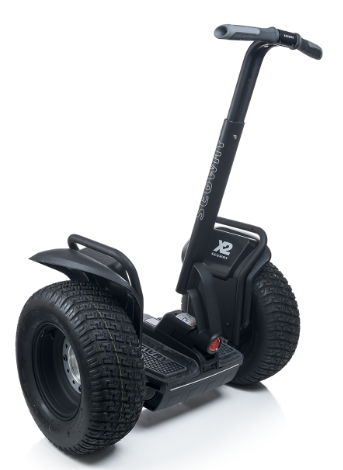
\includegraphics[scale=0.5]{Fundamentos/Segway}
    \caption{Segway X2 SE
    \citep{Segway}.}
    \label{fig:revisao_segway}
\end{figure}

Logo abaixo, segue uma série de trabalhos similares a este aqui proposto. Será descrito de forma breve um pouco sobre os trabalhos em si e a estratégia de controle utilizada, bem como a apresentação da planta física construída.

\subsection{Trabalhos Similares}

O trabalho de \cite{CCEL:17} consistiu na construção de um protótipo projetado por meio de um \textit{software} CAD, visto na Figura (\ref{fig:estadoArte_REF1}), e no desenvolvimento de um sistema de controle para esse projeto. Os autores se engajaram em controlar o sistema com um controlador PID, obtendo seus coeficientes por meio do método de sintonização de \textit{Ziegler-Nichols}. Como sensor utilizaram a placa MPU6050, que possui embutida na mesma o giroscópio e acelerômetro. Contudo, se faz necessário a fusão dos sinais provenientes desses dois sensores para obtenção de uma maior confiabilidade e certeza da medição. Sendo assim, os autores optaram por utilizar o filtro complementar, que nada mais é do que um filtro de média. 
\begin{figure}[H]
    \centering
    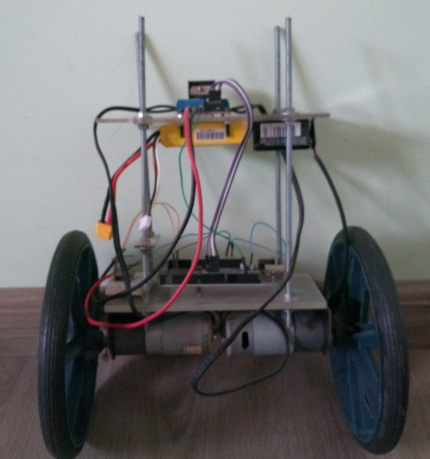
\includegraphics[scale=0.6]{EstadoArte/REF1}
    \caption{Protótipo Pêndulo Invertido
    \citep{CCEL:17}.}
    \label{fig:estadoArte_REF1}
\end{figure}

O artigo de \cite{JVM:17} teve como objetivo a identificação e o controle de um veículo do tipo Segway para fins educacionais. Dessa maneira, o autor dividiu o artigo em partes como: o sistema eletrônico e mecânico, linearização do modelo matemático e discretização, implementação de filtros para a leitura dos sinais provindo do acelerômetro e giroscópio, identificação do sistema e a implementação de um controlador PD (Proporcional-Derivativo), sendo que seus coeficientes foram obtidos por meio de inspeção gráfica utilizando o lugar das raízes. O diagrama de malha fechada padrão, com o controlador em série com o sistema. Os resultados obtidos foram apenas em cima do modelo, sendo assim, não houve a implementação física ou mesmo a montagem do protótipo proposto, como visto na Figura (\ref{fig:estadoArte_REF2}). Os resultados obtidos na simulação foram bem satisfatórios para os critérios adotados, sendo que em malha fechada o autor conseguiu fazer com que o sistema seguisse a referência senoidal aplicada e após aplicação de um distúrbio, o sistema conseguiu se recompor rapidamente.
\begin{figure}[H]
    \centering
    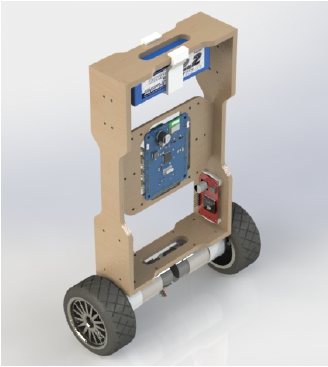
\includegraphics[scale=0.8]{EstadoArte/REF2}
    \caption{Protótipo renderizado
    \citep{JVM:17}.}
    \label{fig:estadoArte_REF2}
\end{figure}

Por último, o artigo de \cite{ME:18} propôs a implementação de um controlador LQR. A modelagem do sistema foi feita utilizando equações lagrangianas e, depois que encontrou uma equação não linear para o sistema, linearizou a mesma e passou para a forma de espaço de estados, chegando assim nas matrizes A, B, C e D. Aplicou a essas matrizes a propriedade de controlabilidade e observabilidade, concluindo assim, que é um sistema controlável e observável. O pêndulo invertido sobre duas rodas, é um sistema de uma única entrada e múltiplas saídas (SIMO). Dessa forma, para lidar com um tipo de sistema desses é mais simples com o LQR baseado pelo controle de velocidade como propôs o autor. Para utilizar esse controlador, é necessário encontrar um vetor de ganhos $K$ e consequentemente, minimizará a função de custo $J$. Na Figura (\ref{fig:estadoArte_REF3.1}) é mostrada a implementação do controlador LQR.
\begin{figure}[H]
    \centering
    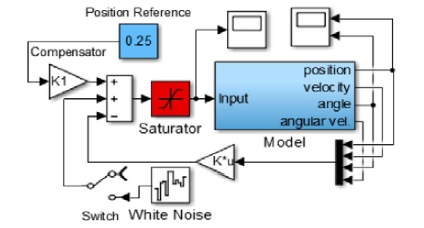
\includegraphics[scale=0.85]{EstadoArte/REF3_1.PNG}
    \caption{Implementação do controlador LQR
    \citep{ME:18}.}
    \label{fig:estadoArte_REF3.1}
\end{figure}

O filtro que foi implementado também foi o complementar, que nada mais é do que um filtro passa-baixas para o acelerômetro e um filtro passa-altas para o giroscópio. As principais variáveis que foram medidas ou estimadas foram: a posição da estrutura, $\theta$, a velocidade angular, $\dot{\theta}$ e, velocidade da roda, $\omega$. O protótipo montado pode ser visto na Figura (\ref{fig:estadoArte_REF3_2}). 
\begin{figure}[H]
    \centering
    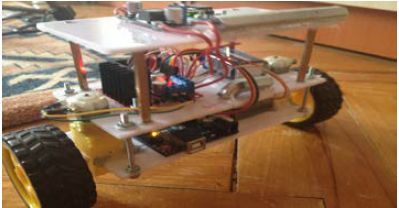
\includegraphics[scale=0.8]{EstadoArte/REF3_2}
    \caption{Planta física construída
    \citep{ME:18}.}
    \label{fig:estadoArte_REF3_2}
\end{figure}

\section{Fundamentos Clássicos da Mecânica}\label{sec:FundamentoClassicosMecanica}

O sistema em estudo conforme já citado é descrito como instável e não linear. Porém para encontrar as equações de movimento que regem o sistema, é preciso escolher algum tipo de método. Para o trabalho em questão, escolheu-se representar o sistema por meio da segunda lei de Newton descrita como sendo
\begin{equation}\label{SegundaLeiNewton}
    \sum \overrightarrow{F_i} = m\overrightarrow{a}
\end{equation}

\begin{equation}\label{SegundaLeiNewtonRotacao}
    \sum \tau_{iz} = J\alpha_z 
\end{equation}
em que os termos do lado esquerdo das Equações (\ref{SegundaLeiNewton}) e (\ref{SegundaLeiNewtonRotacao}) representam todas as forças $(F_i)$ e torques $(\tau)$ que atuam sobre o sistema. Já no lado direito da Equação (\ref{SegundaLeiNewton}), temos a massa total do corpo representada no centro de massa $(m)$ e todas as acelerações lineares $(a)$. Na Equação (\ref{SegundaLeiNewtonRotacao}), as acelerações agora são as angulares representas por $(\alpha_z)$ e o momento de inércia $(J)$ é dado como sendo
\begin{equation}
    J = \sum m_ir_i^2
\end{equation}
em que $m_i$ é a massa e $r$ a distância do objeto até o eixo de rotação.

Um outro fundamento que precisa ser descrito aqui é o cálculo do centro de gravidade (CG) ou centro de massa (CM) de um corpo. Para um sistema tridimensional pode-se definir um vetor posição desse sistema. Sendo uma partícula com coordenadas $x_i$, $y_i$ e $z_i$ seu vetor posição $\overrightarrow{r}$ é definido por
\begin{equation*}\label{eq:eqVetorPosicaoCentroMassa}
    \overrightarrow{r} = x_{cm}\hat{i} + y_{cm}\hat{j} + z_{cm}\hat{k}
\end{equation*}
no qual os vetores $\hat{i}$, $\hat{j}$, $\hat{k}$ são unitários e apontam na direção dos eixos $x$, $y$ e $z$ respectivamente. E finalmente, o cálculo da posição do centro de massa de um sistema de partículas é definido como
\begin{equation}
    \overrightarrow{CM} = \frac{1}{M} \sum\limits_{i=1}^{n} m_i\overrightarrow{r}_i
\end{equation}
em que $M$ é a massa total do sistema.

\section{Linearização}\label{sec:Linearizacao}

Como já dito, o sistema trabalho aqui neste traalho é de natureza não linear. Assim, para que as técnicas clássicas de controle ou mesmo algumas de controle moderno sejam utilizadas nos mesmos é preciso tratá-los por aproximações linearizantes.

Segundo \cite{Ogata}, um sistema para ser denominado de não linear é preciso que o princípio da superposição falhe ao ser aplicado nele. Dessa forma, caso tente obter uma resposta do sistema aplicando duas entradas simultâneas considerando as mesmas individualmente e somando-se os resultados, essa resposta não será válida.

Um sistema representado no espaço de estados é definido por \cite{Hespanha} da seguinte maneira
\begin{equation}\label{eq:DefinicaoSS}
    \begin{array}{cc}
         & \dot{x} = f(x,u) \\[6pt]
         & y = g(x,u)
    \end{array}{}
\end{equation}{}
sendo x $\in \mathbb{R}^{n}$ , y $\in \mathbb{R}^{m}$ e u $\in \mathbb{R}^{k}$.

\subsection{Ponto de equilíbrio}

Para se obter uma aproximação linear de um sistema não linear, é preciso, primeiramente, determinar os pontos de equilíbrio do sistema. A determinação dos pontos de equilíbrio é feito quando se iguala o termo diferencial da Equação (\ref{eq:DefinicaoSS}).

Pela definição de \cite{Hespanha}, têm-se que um par de pontos $(x^{eq},u^{eq})$ $\in$ $\mathbb{R}^n$ x $\mathbb{R}^k$ que pode ser chamado de ponto de equilíbrio de (\ref{eq:DefinicaoSS}) caso $f(x^{eq},u^{eq}) = 0$. A solução de (\ref{eq:DefinicaoSS}) é visto abaixo. 
\begin{equation}
    u(t) = u^{eq}, ~~~~~ x(t) = x^{eq}, ~~~~~ y(t) = y^{eq} := g(x^{eq},u^{eq}), ~~~~~~~~~~ \forall t \ge 0
\end{equation}{}

\subsection{Linearização em torno de um ponto de equilíbrio}\label{subsec:linearizacaoPontoEquilibrio}

De acordo com \cite{Hespanha}, a linearização do sistema em série de Taylor pode ser representado por matrizes Jacobianas, conforme descrito a seguir.

\begin{equation}\label{eq:MatrizesLineares}
    \begin{array}{cc}
         &  A := \dfrac{\partial f(x^{eq},u^{eq})}{\partial x}, ~~~~~~ B := \dfrac{\partial f(x^{eq},u^{eq})}{\partial u},\\[15pt]
         & C := \dfrac{\partial g(x^{eq},u^{eq})}{\partial x}, ~~~~~~ D := \dfrac{\partial g(x^{eq},u^{eq})}{\partial u}
    \end{array}{}
\end{equation}{}

Assim, o sistema linear invariante no tempo (LTI), no espaço de estados, linearizado em torno de um ponto de equilíbrio $(x^{eq},u^{eq})$, é dado por:

\begin{equation}
    \begin{array}{cc}
         &  \dot{\delta x} = A\delta x + B\delta u \\[6pt]
         &  \delta y = C\delta x + D\delta u
    \end{array}{}
\end{equation}{}
em que os termos $\dot{\delta x}(t), \delta{y}(t)$ e $\delta u(t)$ para todo $t \ge 0$ é descrito como
\begin{equation}
    \dot{\delta x}(t) := x(t) - x^{eq}, ~~~~~ \delta y(t) := y(t) - y^{eq}, ~~~~~ \delta u(t) := u(t) - u^{eq} 
\end{equation}{}


\section{Sistema em Espaço de Estados}\label{sec:EspacoEstados}

A representação no espaço de estados garante uma maior facilidade de soluções de um modelo matemático e de um sistema físico, já que a mesma pode relacionar um conjunto de variáveis de entradas, saídas e de estados por meio de equações diferenciais de primeira ordem. A representação fornece de maneira prática as soluções do sistema, por adotar notações matriciais quando o sistema dinâmico é linear e invariante no tempo.

\subsection{Caso contínuo no tempo}

No caso contínuo no tempo, um sistema representado no espaço de estados de acordo com \cite{Hespanha} pode ser descrito como
\begin{equation} \label{eq:SSContinuo}
    \begin{array}{cc}
         & \dot{x}(t) = A(t)x(t) + B(t)u(t) \\[6pt]
         & y(t) = C(t)x(t) + D(t)u(t)
    \end{array}{}
\end{equation}{}
no qual os sinais $u$, $y$ e $x$ das Equação (\ref{eq:SSContinuo}) são chamados de entrada, saída e de estados respectivamente e definidos por
\begin{equation*}
    \begin{array}{c}
        u:[0,\infty] \rightarrow \mathbb{R}^k, ~~~~~~~
        x:[0,\infty] \rightarrow \mathbb{R}^n, ~~~~~~~
        y:[0,\infty] \rightarrow \mathbb{R}^m
    \end{array}{}
\end{equation*}{}

Sendo o sistema representado pela Equação (\ref{eq:SSContinuo}) linear e as matrizes A(t), B(t), C(t) e D(t) constantes $\forall t \ge 0$, o sistema  é chamado de linear invariante no tempo (LTI). Assim, pode-se simplificar a representação no caso contínuo
\begin{equation}\label{eq:SSContinuoLTI}
    \begin{array}{cc}
         & \dot{x}(t) = Ax(t) + Bu(t) \\[6pt]
         & y(t) = Cx(t) + Du(t)
    \end{array}{}
\end{equation}{}

As dimensões das matrizes $A$, $B$, $C$ e $D$ das Equações (\ref{eq:SSContinuo}) e (\ref{eq:SSContinuoLTI}) são as mesmas e são definidas como sendo
\begin{equation*}
    \begin{array}{cc}
    &    A \in \mathbb{R}^{n \times n} ~~~~~~~
         B \in \mathbb{R}^{k \times m}  \\[6pt]
    &    C \in \mathbb{R}^{l \times n} ~~~~~~~
         D \in \mathbb{R}^{l \times m}
    \end{array}{}
\end{equation*}{}


\subsection{Caso discreto no tempo}

As aplicações de forma geral são feitas utilizando microcontroladores ou algum dispositivo digital. Sendo assim, para aplicações desse tipo, faz-se necessário a discretização do sistema. 

\cite{Chen} afirma que a representação discreta do sistema no espaço de estados é descrita como
\begin{equation}
    \begin{array}{cc} \label{eq:SSDiscretoLTI}
         & x_{k+1} = A_dx_k + B_du_k \\[6pt]
         & y_k = C_dx_k + D_du_k
    \end{array}{}
\end{equation}{}
em que a variável $t=kT$ com $k=0,1,2,..,k_f$ e $T$ o período de amostragem do sistema. O período é escolhido de forma a ser o menor possível, ou seja, o máximo que o microcontrolador consegue trabalhar. As matrizes $A_d$, $B_d$, $C_d$, $D_d$ são descritas como se segue bem como a solução para $A_d$ e $B_d$ \citep[p. 91]{Chen}
\begin{equation}\label{eq:MetodoDiscretizacao}
    A_d = e^{AT} ~~~~~ B_d = \left(\int_{0}^{T} e^{A\tau} \, d\tau\right)B~~~~~  C_d = C ~~~~~ D_d = D    
\end{equation}


\section{Realimentação de Estados}

Uma das formas de se implementar controladores por meio da representação no espaço de estados é por meio da realimentação de estados, no qual utiliza-se os próprios estados do sistema com um fator multiplicativo (ganho) para gerar o sinal de controle. Para ter acesso a todos os estados da planta deve-se ter sensores para cada um dos estados do sistema. Como na maioria das aplicações reais isso não ocorre, pois implica em um custo elevado, faz-se necessário a implementação de um sistema que irá estimar os estados (observador) e assim, o sinal de controle passará a ser com relação a esses estados estimados. Contudo, para realizar a construção de um observador ou mesmo fazer o controle do sistema, deve-se, primeiramente, testar o sistema com métodos matemáticos que informam tais capacidades. Dito isso, os critérios são apresentados a seguir para um sistema discreto
\begin{equation}\label{eq:SSDiscretoLTI2}
    \begin{array}{cc}
         &  x_{k+1} = A_dx_k + B_du_k \\[10pt]
         &  y_k = C_dx_k + D_du_k
    \end{array}{}
\end{equation}{}

\subsection{Controlabilidade}

De acordo com \cite{Hespanha}, para saber se o sistema é controlável ou não, utiliza-se as matrizes $A_d$ e $B_d$ da equação de estados de (\ref{eq:SSDiscretoLTI2}). O critério para determinar a controlabilidade é demonstrado como sendo
\begin{equation}\label{eq:Controlabilidade}
\mathbb{C} := \left[\begin{array}{ccccc}
        B_d & A_dB_d & A_d^2B_d & \dots & A_d^{n-1}B_d
     \end{array}\right]_{n\times(kn)} 
\end{equation}{}

A partir do critério (\ref{eq:Controlabilidade}) pode-se determinar se o sistema em questão poderá ou não ser controlável. Segundo \cite{Ogata}, para que o sistema seja controlável é preciso que o determinante da matriz (\ref{eq:Controlabilidade}) seja diferente de $0$, ou seja, que tenham vetores linearmente independentes (LI) e assim, posto $n$.

\subsection{Observabilidade}

Como não haverá medições diretas de todos os estados, será necessário a utilização de um observador como já mencionado. O mesmo irá estimar o valor dos estados que faltam e assim a lei de controle da realimentação será baseado neles. 

Contudo, nem todos os sistemas são observáveis, dessa forma é preciso garantir que o sistema deste trabalho seja observável. De acordo com \cite{Hespanha}, o critério no qual testa-se o sistema será observável ou não é mostrado como sendo
\begin{equation}\label{eq:Observabilidade}
\mathbb{O} := \left[\begin{array}{c}
        C_d ~ \\ C_dA_d ~ \\ C_dA_d^2 ~ \\ \vdots ~ \\ C_dA_d^{n-1}
    \end{array}\right]_{(kn) \times n}
\end{equation}\\

A análise da matriz (\ref{eq:Observabilidade}) é dual ao critério de controlabilidade. Para que o sistema seja observável é preciso que os vetores sejam LI, ou seja, que tenham posto ($\textit{rank}$) igual a $n$.

\section{Controlador Linear Gaussiano Quadrático (LQG)}\label{sec:MetodologiaControladorLQG}

De acordo com \cite{Steven:17}, o controlador LQG é constituído por um estimador quadrático linear (LQE) ou mais popularmente denominado de Filtro de Kalman, ou seja, um observador no qual os estados estimados são realimentados através de ganhos ótimos projetados por meio do regulador linear quadrático (LQR). A Figura (\ref{fig:controladorLQG}) apresenta como deve ser o \textit{design} de um controlador LQG.
\begin{figure}[H]
    \centering
    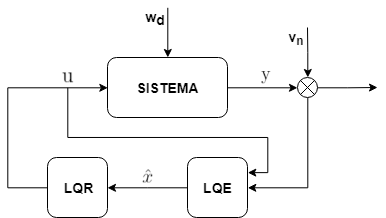
\includegraphics[scale=0.75]{Fundamentos/LQG}
    \caption{Estrutura de um controlador LQG.}
    \label{fig:controladorLQG}
\end{figure}

\subsection{Regulador Linear Quadrático  (LQR)}\label{subsec:MetodologiaControladorLQR}

O LQR possui como principal característica a garantia de estabilidade em malha fechada, um alto grau de robustez do sistema controlado proporcionado ao mesmo margem de ganho infinita e margem de fase $\pm 60^\circ$ \citep{Fernandes:14}. Contudo, se faz necessário conhecer todos os estados do sistema para se trabalhar com este regulador. Dessa maneira, é usual utilizar este controlador juntamente com um estimador tal como o LQE.

Para encontrar o ganho ótimo do LQR, considera-se o seguinte sistema no tempo discreto.
\begin{equation}
    \begin{array}{cc}
         &  x_{k+1} = A_dx_k + B_du_k \\[6pt]
         &  y_k = C_dx_k
    \end{array}{}
\end{equation}{}

Assume-se que $x(0) = x_0$ e $k = 0, 1, 2,\dots,k_f$. De acordo com \cite{Sage}, a função de custo a ser minimizada é dada por:
\begin{equation}\label{eq:FuncaoCustoLQR}
    J = \frac{1}{2}||x_{k_f}||^2_S + \frac{1}{2}\sum_{k=0}^{k_f-1} \{||x_k||^2_Q + ||u_k||^2_R\}
\end{equation}{}

A matriz $Q \in \reais^{nxn}$ é uma matriz positiva semi-definida e $R \in \reais^{mxm}$ é uma matriz positiva definida. Essas matrizes são responsáveis pela ponderação dos estados e o sinal de controle do sistema. De acordo com \cite{Matos:08}, essas matrizes são escolhidas da seguinte forma:
\begin{equation*}
    \begin{array}{cc}
         &  Q = C_d^TC_d\\[6pt]
         &  R = \rho \I_{mxm}, ~~~ \rho > 0.
    \end{array}{}
\end{equation*}{}

Conforme \cite{Sage}, a equação Hamiltoniana é dada como se segue.
\begin{equation}\label{eq:Hamiltoniana}
    H_k = \frac{1}{2}x_k^TQx_k + \frac{1}{2}u_k^TRu_k + \lambda_{k+1}^T[A_dx_k + B_du_k]
\end{equation}{}

Caso o par $(A_d,B_d)$ seja controlável e o par $(A_d,C_d)$ observável, a lei de controle ótimo que minimiza a equação de custo (\ref{eq:FuncaoCustoLQR}) é dada por:
\begin{equation}\label{eq:LeiControleLQR}
    u_k = -Kx_k
\end{equation}{}
em que a matriz $K \in \mathbb{R}^{mxn}$ de ganhos ótimos do controlador LQR é definida como se segue
\begin{equation}\label{eq:GanhoLQR}
    K = (R + B_d^TPB_d)^{-1}B_d^TPA_d
\end{equation}{}
no qual a matriz simétrica $P \in \mathbb{R}^{nxn}$ é conseguida após solucionar a equação de Riccati de forma recursiva como segue
\begin{equation}\label{eq:RiccatiLQR}
    P_{k+1} = Q + A^TP_kA_d - A_d^TP_kB_d(R + B_d^TP_kB_d)^{-1}B_d^TP_kA_d
\end{equation}{}

\subsection{Estimador de Estados Quadrático (LQE)}\label{sec:MetodologiaFiltroKalman}

\cite{Sundin:12} afirmam que os o filtro capaz de fazer a estimação da derivada do giroscópio é o Filtro de Kalman. O Filtro de Kalman surgiu da teoria de otimização e é um estimador ótimo para sistemas que possuem distúrbios e apresentam características de distribuição normal de ruído branco. O filtro modela o comportamento do sensor e isso inclui o $\textit{bias}$ que possa vir a ter, o que dá uma boa estimativa do ângulo e do $\textit{bias}$ do giroscópio, que melhora a taxa angular uma vez que o mesmo pode ser removido. A Figura (\ref{fig:estimadorLQE}) apresenta a estrutura do filtro no tempo discreto.
\begin{figure}[H]
    \centering
    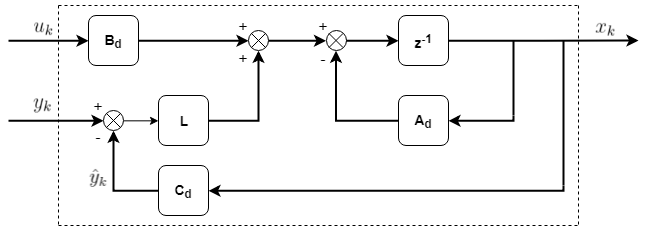
\includegraphics[scale=0.6]{Fundamentos/Kalman}
    \caption{Estrutura do Filtro de Kalman discreto em Espaço de Estados. Adaptado de \cite{Steven:17}.}
    \label{fig:estimadorLQE}
\end{figure}

O ganho do estimador ótimo quadrático linear se baseia no desempenho do observado projetado com a presença de erro de medição e ruído de processo. Logo, a cada tempo que passa o ganho do filtro de Kalman vai sendo atualizado. Primeiramente, para realizar o projeto desse estimador considera-se o seguinte sistema
\begin{equation}\label{eq:SistemaLQE}
    \begin{array}{cc}
         &  x_{k+1} = A_d x_k + B_d u_k + w_k\\[6pt]
         &  y_k = C_dx_k + v_k
    \end{array}{}
\end{equation}{}
em que o ruído $w_k$ e o erro de medição $v_k$ são sequências aleatórias de ruído branco gaussiano com média zero \cite[p. 231]{Sage}. Sendo assim, temos
\begin{equation*}
    \mathbb{E}\{w_k\} = 0 ~~~ \text{e} ~~~ \mathbb{E}\{v_k\} = 0 
\end{equation*}{}
em que $\mathbb{E}\{\}$ é conhecido como expectância ou valor esperado. A correlação por se tratar de ruído branco é zero 
\begin{equation*}
    cov\{w_iw_j^T\} = 0 ~~~ \text{e} ~~~ cov\{v_iv_j^T\} = 0 ~~~ \text{para} ~~~ i \ne j
\end{equation*}{}
e a covariância é definida por
\begin{equation*}
    cov\{w_kw_k^T\} = Q_o ~~~ \text{e} ~~~ cov\{v_kv_k^T\} = R_o
\end{equation*}{}

A principal tarefa da otimização é determinar uma matriz de ganhos que minimizará a variância da estimação do erro, que é denotado por $G_k$
\begin{equation}\label{eq:VarianciaEstimacao}
    G_k = \mathbb{E} \{(x_k-\hat{x}_k)(x_k-\hat{x}_k)^T\}
\end{equation}{}

Segundo \cite{Steven:17}, um estimador produz uma estimação dos estados $x_k$ conhecida como $\hat{x_k}$ caso conheça a saída medida $y_k$ provinda de um sensor e o sinal de entrada $u_k$. Caso o sistema seja observável, é possível construir o filtro a partir do ganho $L$ como se segue
\begin{equation}\label{eq:DinamicaEstimadorLQE}
    \begin{array}{cc}
        &  \hat{x}_{k+1} = A_d \hat{x}_k + B_d u_k + L_k(y_k - \hat{y}_k) \\
        &  \hat{y}_k = C_d\hat{x}
    \end{array}{}
\end{equation}{}
sendo que a saída $\hat{y}_k$ é a predição da expectativa da saída do sensor baseada no estados estimados $\hat{x}_k$. Manipulando a Equação
(\ref{eq:DinamicaEstimadorLQE}), encontra-se uma expressão para $\hat{x}_{k+1}$.
\begin{align}
     \hat{x}_{k+1} & = (A_d - LC_d)\hat{x}_k + B_du_k + Ly_k \nonumber \\ 
                   & = (A_d - LC_d)\hat{x}_k + \left[\begin{array}{cc}
                                            B_d & L
                                            \end{array}{}\right]    \left[\begin{array}{cc}
                                        u_k\\
                                        y_k
                                    \end{array}{}\right]
\end{align}
assim, as matrizes $A_f$ e $B_f$ do filtro de Kalman são:
\begin{align}\label{eq:MatrizesFiltroKalman}
    \begin{array}{cc}
        A_f = \left(\begin{array}{c}                   
                    A_d - LC_d
                \end{array}\right) ~~~~~~~~~~~
        B_f = \left[\begin{array}{cc}
                 B_d & L 
              \end{array}\right]
    \end{array}{}
\end{align}{}

De acordo com \cite{Kim:13}, o ganho $L$ do filtro de Kalman é um vetor pertencente aos números reais e de dimensão n$\times$1 e é definido pela seguinte expressão
\begin{equation}\label{eq:Ganho1LQE}
    L = A_dS_kC_d^T(C_dSC_d^T + R_o)^{-1}
\end{equation}{}
na qual a matriz S é obtida quando soluciona-se a equação de Riccati
para a equação de diferenças. A expressão que precisa-se solucionar e que fará com que o ganho $L$ seja ótimo é descrita como
\begin{equation}\label{eq:MatrizMinimizaçãoLQE}
    S_{k+1} = Q_o + A_dS_kA_d^T - A_dS_kC^T(C_dS_kC_d^T + R_o)^{-1}C_dS_kA_d^T
\end{equation}{}
em que $Q_o$ é uma matriz positiva definida e $R_o > 0$ são especificados como parâmetros de projeto, considerando a condição inicial $S_0 = 0$.










\begin{comment}

\section{Filtros}\label{sec:Filtros}

Em grande parte de sistemas que utilizam de sensores necessitam de algum tipo de filtro. E nesta seção dois filtros testados e aplicados no sistema serão explicados.

Primeiramente, para um boa estimação da inclinação do pêndulo é necessário que os sinais de leitura do acelerômetro e do giroscópio sejam fundidos com objetivo de criar um novo sinal mais estável e fidedigno. Segundo \cite{Sundin:12}, os sensores possuem diferentes propriedades que afetam a estimação do ângulo de diferentes maneiras. Abaixo é listado as principais de cada.
\begin{itemize}
    \item \textbf{Acelerômetro}: o acelerômetro tem uma boa leitura da inclinação da estrutura quando outras forças não atuam sobre ele tais como movimentos lineares. Para se conseguir uma estimativa correta é necessário que apenas a força da gravidade esteja atuando sobre o sensor ou então o mesmo não retornará uma leitura fiel do ângulo.

    \item \textbf{Giroscópio}: o giroscópio tem uma boa estimativa do ângulo \textit{pitch}, $\theta$, realizando a integral da saída de interesse, ou seja, da inclinação do sistema. Esse ângulo não é afetado por forças lineares pela movimentação do robô mas o sensor pode ter sua leitura comprometida caso o mesmo apresente algum \textit{bias} (ou \textit{offset}) que fará com que sua leitura não seja a verdadeira.
\end{itemize}

Utilizando os conhecimentos a respeito de filtros os mesmos podem ser utilizados para obter uma resposta mais confiável então da leitura do ângulo. Dessa maneira, abaixo será descrito dois filtros utilizados no sistema que fazem a fusão dos sensores.

\subsection{Filtro Complementar}

O filtro complementar é em sua maior parte utilizada em projetos $\textit{hobbistas}$ por ser simples e um bom filtro de fusão para dois sensores. O filtro possui fácil implementação e de ajuste experimental e demanda pouco poder de processamento \citep{Sundin:12}. Por ser formado por dois fitros, passas altas e passas baixas, cada um atua em um sensor, sendo que o primeiro atua no giroscópio e o segundo no acelerômetro. O ângulo $\theta$ é dado pela seguinte maneira
\begin{equation}
    \theta_k = (1 - \alpha)(\theta_{k-1} + \dot{\theta}_{k,gyro}dt) + \theta\alpha_{k,acc}
\end{equation}
em que $dt$ é o tempo de amostragem e $\alpha$ é a constante do filtro. Então, para extrair o que este filtro tem de melhor, é necessário ajustar a contante $\alpha$ até que o resultado seja bom, o que faz a constante de tempo do filtro alterar e consequentemente o $\textit{bias}$ do giroscópio é removido. Por mais que este filtro pareça ser excelente por todas as vantagens apresentadas, o mesmo apresenta desvantagens tal como não saber o $\textit{bias}$ real do giroscópio e assim dará apenas uma boa estimativa do ângulo.

\section{PWM}\label{sec:PWM}
Uma vez que o sistema será alimentado por uma bateria, a mesma fornece uma tensão constante e para poder variar a velocidade dos motores é preciso controlar a tensão. Assim, para esta modulação foi utilizado uma técnica simples de baixas perdas energéticas e que tem suporte do \textit{hardware} e \textit{software} no Arduino \textbf{CITAR SUSAN}. Dessa forma, a energia é drenada da bateria e ligada e desligada pelo controlador dos motores. Devido a inércia elétrica, a tensão não atingirá o zero volts e nem ao máximo entre cada período de comutação, mas em vez disso, estará próximo da média resultante dependendo do ciclo de trabalho (\textit{Duty Cicle}) $D$. A tensão de saída do PWM é descrita como
\begin{gather}
    U = \frac{1}{T}\int_{0}^{T} f(t)\, dt
\end{gather}
e $f(t)$ é uma função de pulso descrita como sendo
\begin{equation}
f(t) = 
    \left \{
        \begin{array}{cc}
            U_{max}, & \mbox{se } 0 < t \leq D\times T \\
            0      , & \mbox{se } D\times T < t \leq T \\
        \end{array}
    \right.
\end{equation}
que por sua vez produz uma tensão média que pode ser calculada como
\begin{equation}
    U = D \times U_{max}
\end{equation}

A Figura (\ref{fig:PWM}) explica graficamente a função $f(t)$.
\begin{figure}[!htb]
    \centering
    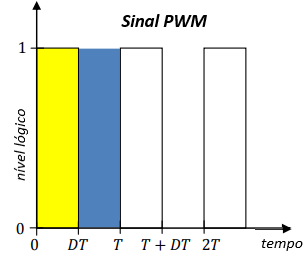
\includegraphics[scale=0.8]{Metodologia/PWM}
    \caption{Gráfico que demonstra o funcionamento do sinal PWM. A parte colorida de amarelo é o sinal em alta ou quando o sinal está ligado e em azul o oposto.}
    \label{fig:PWM}
\end{figure}

\end{comment}


\chapter{Sistema Mecatrônico}\label{cap:Metodologia}

De maneira geral, a estrutura do robô possui forma retangular com duas rodas. As rodas são acopladas de forma que fiquem paralelas uma a outra. A estrutura pode ser comparada como uma estante, no qual o mesmo foi projetado para três e em cada uma delas estão alguns componentes.  A Figura (\ref{fig:EstruturaRealVisaoFrontalLateral}) mostra a vista isométrica da estrutura.
\begin{figure}[H]
    \centering
    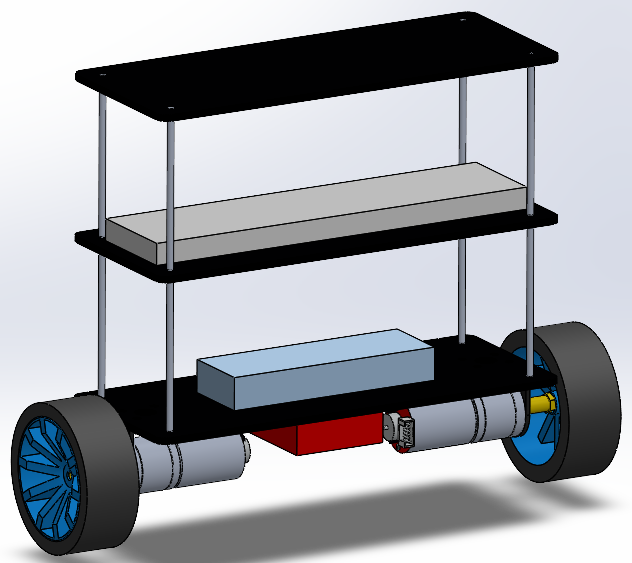
\includegraphics[scale=0.6]{Metodologia/Pendulo_3D.PNG}
    \caption{Estrutura real do pêndulo na visão frontal e lateral.}
    \label{fig:EstruturaRealVisaoFrontalLateral}
\end{figure}

\section{Estrutura Adotada}\label{sec:EstruturaCAD}

A estrutura do pêndulo consiste em quatro barras rosqueadas que serve para sustentar as prateleiras em seus devidos lugares. O material utilizado para fazer as bases do pêndulo foi o ACM. Foi adotado uma altura de 200 $mm$ para a planta medindo do chão ao topo, a largura de 80 $mm$ que é o padrão das placas com uma espessura de 3 $mm$. 
Os componentes do sistema foram distribuídos em cada andar. Na parte inferior da primeira estante ou no ponto mais próximo ao solo temos o \textit{driver} dos motores e os motores propriamente dito. Contudo, foi necessário a utilização de um suporte que fixasse os motores a base. Já no segundo andar ou na segunda prateleira, estão o microprocessador Arduino Nano e o sensor que capturará o ângulo de inclinação da planta. Por fim, para deixar o centro de massa um pouco mais distante do eixo de referência que passa entre os motores, posicionou-se a bateria na última placa. Em muitas literaturas aconselha-se adotar esse tipo de estratégia para facilitar o controle do pêndulo invertido.

\subsection{Parâmetros Mecânicos da Estrutura}

A Tabela (\ref{tab:ParametroEstrutura}) apresenta os parâmetros mecânicos da estrutura do pêndulo bem como seus respectivos valores. Tais parâmetros foram medidos ou mesmo calculados como mostra o Apêndice ().
\begin{table}[!htb]
\centering
\caption{Parâmetros mecânicos obtidos através de medições práticas e via cálculos.}
\label{tab:ParametroEstrutura}
\begin{tabular}{@{}cccc@{}}
\toprule
\textbf{Descrição da grandeza} & \multicolumn{1}{l}{\textbf{Variável}} & \textbf{Valor Nominal} & \textbf{Unidade de medida} \\ \midrule
Momento de Inércia do Pêndulo           & $J_p$         & 0.00530429    & $kg.m^2$    \\
Momento de Inércia das Rodas            & $J_w$         & 0.00005013    & $kg.m^2$    \\
Massa total da planta física            & $m$           & 0.7740        & $kg$      \\
Massa do pêndulo s/rodas                & $M_{p}$       & 0.7120        & $kg$      \\
Massa de duas rodas                     & $M_{r}$       & 0.0620        & $kg$      \\
Altura do centro de massa ao eixo    & $z_{cm}$      & 0.0836        & $m$         \\
Raio externo das rodas                  & $r_{ext}$     & 0.0315        & $m$         \\
Raio interno das rodas                  & $r_{int}$     & 0.0250        & $m$         \\
Distância eixo até o conjunto-placa 1   & $d_{h1}$      & 0.0150        & $m$       \\
Distância eixo até o conjunto-placa 2   & $d_{h2}$      & 0.120         & $m$       \\
Distância eixo até o conjunto-placa 3   & $d_{h3}$      & 0.180         & $m$       \\
Distância do chão até o topo            & $H$           & 0.200         & $m$       \\
Largura dos conjuntos-placa             & $W$           & 0.080         & $m$       \\
Resistência de armadura do motor        & $R$           & 0.91          & $\Omega$  \\
\bottomrule
\end{tabular}
\end{table}

\section{Instrumentação}

No momento em que se inicia o planejamento de um projeto de engenharia, é de suma importância
realizar a listagem dos recursos que serão utilizados, bem como a justificativa de cada. Desta
forma, segue abaixo a listagem dos \textit{softwares} e materiais que foram ordenados da seguinte maneira: atuadores, transdutor de orientação e eletrônica.

\subsection{Arduino Nano}

O Arduino Nano é um microcontrolador de baixo custo e de alta performance. Essa placa será responsável por realizar o controle do sistema, fazer a leitura dos sinais do sensor e enviar os sinais de controle para o atuador. A placa pode ser vista na Figura (\ref{fig:ArduinoNano}).
\begin{figure}[H]
    \centering
    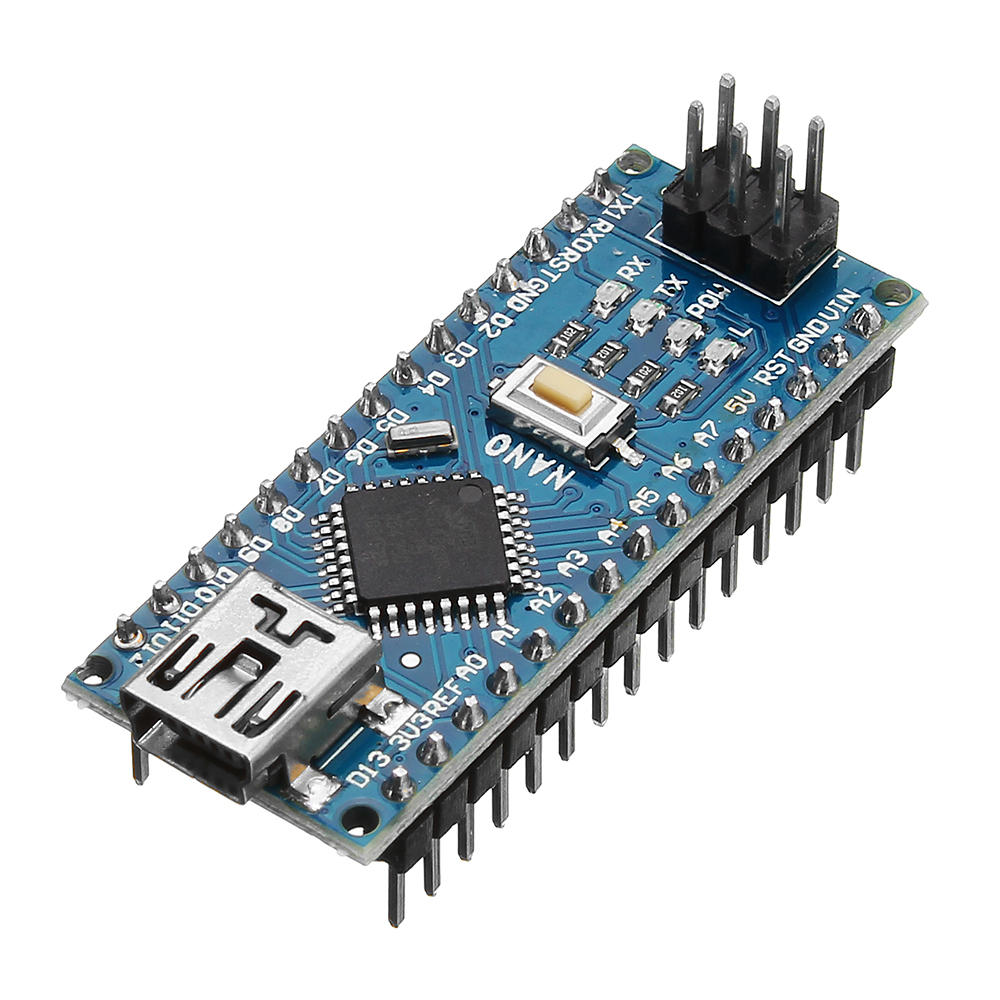
\includegraphics[scale=0.15]{Metodologia/arduinoNano}
    \caption{Visão da placa responsável pela leitura dos sinais do sensor e processamento dos sinais de controle.}
    \label{fig:ArduinoNano}
\end{figure}

A decisão da utilização dessa placa ao invés de outro microcontrolador seu deu pelo fato de que a mesma conseguiria suprir os requisitos para o projeto, como a quantidade mínima de pinos PWM e digitais e a capacidade de processamento dos dados. A partir do \textit{datasheet} da placa, é possível conhecer as características principais que a compõe, como visto abaixo.
\begin{table}[!htb]\label{tab:CaracteristicaArduinoNano}
\centering
\caption{Dados do fabricante sobre a placa Arduino Nano.}
\begin{tabular}{lc}
\hline
\textbf{Descrição}               & \textbf{Valores Nominais}    \\ \hline
Chip                             & ATmega328P – 8 bit AVR       \\
Tensão de Operação               & 5 $V_{cc}$                   \\
Tensão de Alimentação $(V_{in})$ & 7$\sim$12 $V_{cc}$             \\
Pinos Digitais                   & 14 (D0 - D13)                \\
Pinos Digitais PWM               & D3, D5, D6, D9, D11 (8 bit)  \\ 
Pinos Analógicos                 & 8 (A0 - A7)                  \\
Corrente Máxima p/Pino           & 40 $mA$                      \\
Memória Flash                    & 32 $kB$                      \\
Clock                            & 16 $MHz$                     \\ \hline
\end{tabular}
\end{table}

\subsection{Driver Motor CC}

A Figura (\ref{fig:PonteH}) apresenta o \textit{driver} do motor CC que será utilizado, a Ponte H L298N. Com essa placa será possível realizar o controle de sentido de giro e realizar o controle da velocidade dos dois motores por meio de sinais PWM ($\textit{Pulse Width Modulation}$).
\begin{figure}[H]
    \centering
    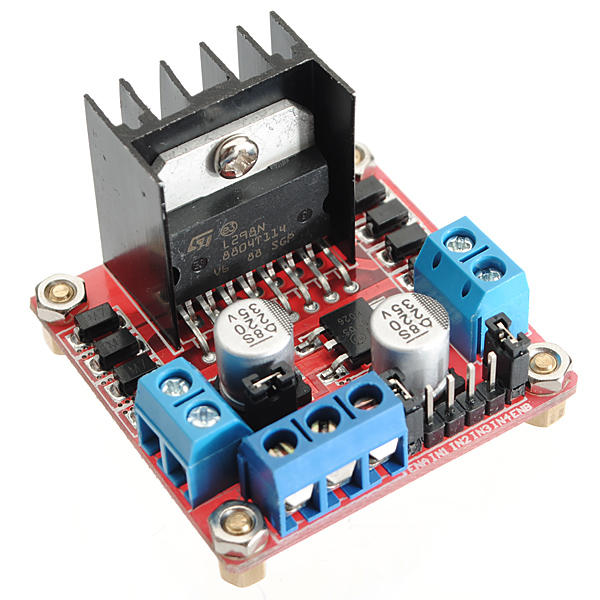
\includegraphics[scale=1]{Metodologia/L298N}
    \caption{Visualização comercial do \textit{driver} Ponte H L298N.}
    \label{fig:PonteH}
\end{figure}

Todas as características dessa placa se encontram na folha de dados do fabricante e algumas das mais importantes a serem consideradas podem ser vistas na Tabela (\ref{tab:CaracteristicaMPU}).
\begin{table}[!htb]\label{tab:CaracteristicaMPU}
\centering
\caption{Parâmetros mecânicos da estrutura.}
\begin{tabular}{lc}
\hline
\textbf{Descrição}              & \textbf{Valores Nominais}   \\ \hline
Tensão de Operação              & 4$\sim$35 $V_{cc}$          \\
Tensão Lógica                   & 5$V$                        \\
Corrente de Operação Máxima     & 2$A$ por canal              \\
Corrente Lógica                 & 0$\sim$36 $mA$              \\
Dimensões (C$\times$L$\times$A) & 43$\times$43$\times$27 $mm$ \\ \hline
\end{tabular}
\end{table}

Como mencionado, com essa placa realiza-se duas coisas importantes, mudança no sentido de giro e a alteração da velocidade dos motores. O primeiro caso é realizado mudando o sentido da corrente, pois os motores CC giram a partir de um campo magnético que é provocado por uma corrente que passa em suas bobinas. Já no segundo caso temos a variação de velocidade por meio do sinal PWM, na qual a tensão de saída que chegará nos terminais do motor será uma tensão média que sempre dependerá do ciclo de trabalho daquele instante.

Como mencionado, com essa placa realiza-se duas coisas importantes, mudança no sentido de giro e alteração da velocidade dos motores. O primeiro caso é realizado mudando o sentido da corrente, pois os motores CC giram a partir de um campo magnético que é provocado por uma corrente que passa em suas bobinas.

Para controlar a velocidade do motor, é necessário recorrer ao PWM, que nada mais é do que uma técnica que obtém resultados analógicos por meio digitais. A técnica consiste em ondas quadradas de alta frequência das quais é possível controlar o percentual de tensão que é aplicado aos motores. Para realizar isto, basta controlar o tempo que deseja manter a saída em 1 (ou ligado) e o em 0 (ou desligado). Esse tempo em nível alto é chamado de $\textit{Duty Cicle}$ e ao utilizar desse recurso, o valor médio de tensão aplicado aos terminais do motor será alterado. 

A partir da Figura (\ref{fig:PWM}), é possível obter a equação do $\textit{Duty Cicle}$ (DC) e da tensão média que será de fato o valor aplicado aos motores.
\begin{equation}
    \begin{array}{cc}
         &  DC = \dfrac{DT}{T}\\[20pt]
         &  U_{medio} = U_{max}(DC)
    \end{array}{}
\end{equation}{}

\begin{figure}[!htb]
    \centering
    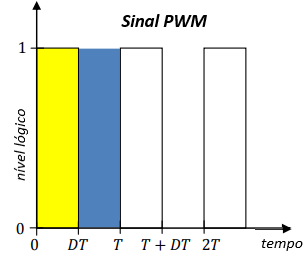
\includegraphics[scale=1]{Metodologia/PWM}
    \caption{Representação de um sinal PWM.}
    \label{fig:PWM}
\end{figure}

\subsection{Atuador}

A Figura \ref{fig:KitMotor} mostra o atuador da planta escolhido juntamente com seus componentes complementares. O motor é responsável por receber o sinal do controle e transformar em tração, movimentando assim o pêndulo.
\begin{figure}[!htb]
    \centering
    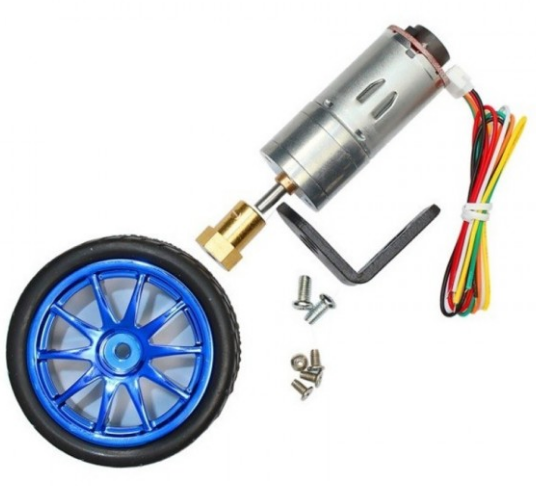
\includegraphics[scale=0.45]{Metodologia/KitMotor}
    \caption{Conjunto completo do atuador composto por motor, roda, suporte de acoplamento da roda ao motor, suporte de acoplamento do motor à base e parafusos.}
    \label{fig:KitMotor}
\end{figure}

\subsubsection{Motores}

O motor escolhido em questão opera com uma tensão de 6V contínuo com uma taxa de redução de 34:1 que faz com tenha pouco \textit{backlash}. Possui encoder de quadratura acoplado na parte anterior de resolução de 11 pulsos por resolução no eixo do motor, que corresponde a 341.2 pulsos por resolução na saída após a caixa de redução. Normalmente, motores pequenos e de baixo preços costumam não possuir uma folha de dados completa e, portanto, as constantes dos mesmo são desconhecidas. Mas nas especificações disponíveis há a tensão nominal ou de operação, velocidade e corrente sem carga, torque, velocidade, potência e corrente em máxima eficiência. Como o motor é de polos é possível encontrar resistência de armadura de forma direta medindo por meio de um multímetro seus terminais. Neste dois casos desconsidera indutância por se tratar de um valor muito pequeno e sua influência será praticamente nula \cite{Sundin:12}.

\begin{table}[!htb]\label{tab:ParametrosDatasheetMotor}
\centering
\caption{Dados do fabricante em relação ao motor.}
\begin{tabular}{lc}
\hline
\textbf{Condições}       & \textbf{Valores Nominais}              \\ \hline

Tensão Operação          & 6 $V_{cc}$                           \\
Resistência de armadura  & 8 $\Omega$                           \\
Velocidade Sem Carga     & 210$RPM$ (0.13$A$)                       \\
Eixo Travado             & 0.980665$Nm$ (3.2$A$)                    \\
Máxima Eficiência        & 0.196133$Nm$ / 170$RPM$ / 2.0$W$ / 0.60$A$     \\
Máxima Potência          & 0.509946$Nm$ / 110$RPM$ / 3.1$W$ / 1.10$A$ \\
Taxa de Redução          & 34:1                                 \\
 
\hline
\end{tabular}
\end{table}

\subsubsection{Rodas}

O conjunto roda e pneus utilizados possuem dimensão de 65$\times$25$mm$. As rodas foram escolhidas desse tamanho por considerar que as mesmas atendem a velocidade angular do motor e a velocidade desejada para o sistema. Por sua vez, a roda é fabricada por um tipo de plástico azul brilhante e os pneus por borracha. O conjunto é acoplado ao motor através de um suporte e fixado por um parafuso bem no centro da roda. O conjunto será aproximado por por um anel para o cálculo do momento de inércia e não por um cilindro maciço já que as rodas é vazada e possuem alguns rasgos.
\begin{table}[!htb]\label{tab:ParametrosRoda}
\centering
\caption{Parâmetros da roda obtidos experimentalmente.}
\begin{tabular}{@{}cccc@{}}
\toprule
\textbf{Parâmetro} &\textbf{Valor Nominal} &\textbf{Unidade} &\textbf{Descrição}       \\ \midrule

\textbf{$M_r$}     & 0.0310         & $kg$            & Massa de cada roda       \\
\textbf{$r_{1}$}       & 0.0250         & $m$             & Raio interno da roda             \\
\textbf{$r_{2}$}       & 0.0315         & $m$             & Raio externo da roda             \\
\bottomrule
\end{tabular}
\end{table}

\subsection{Transdutor de Orientação}

Essa $\textit{shield}$ possui dois sensores, acelerômetro e giroscópio, dos quais serão fundidos a fim de obter uma melhor precisão da medição da orientação da estrutura do pêndulo. A Figura (\ref{fig:MPU6050}) apresenta a placa física e um modelo que representa todos os 6 eixos, 3 para o acelerômetro e 3 para o giroscópio, o que faz com a mesma possua 6 graus de liberdade ($\textit{6DOF}$). 
\begin{figure}[H]
    \centering
    \subfigure[\label{PlacaMPU6050}]{
    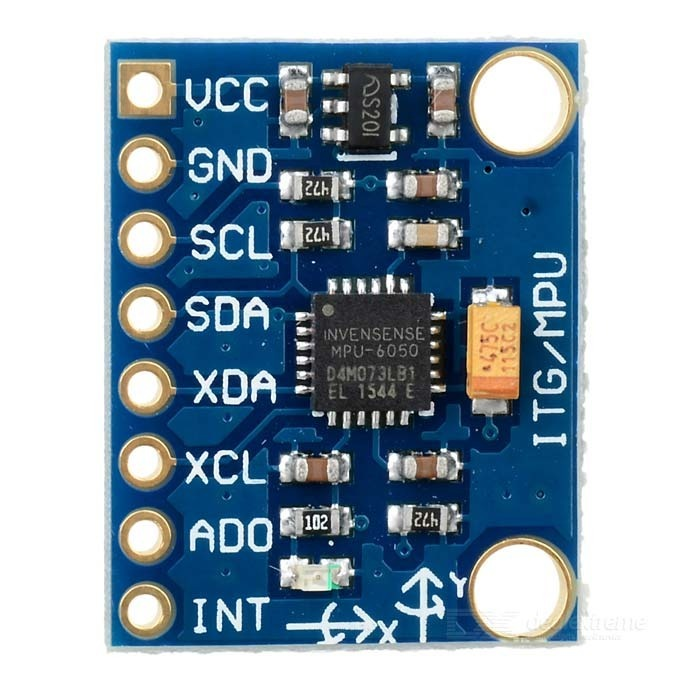
\includegraphics[scale=0.13]{Metodologia/MPU6050}}
    \subfigure[\label{MPUEixos}]{
    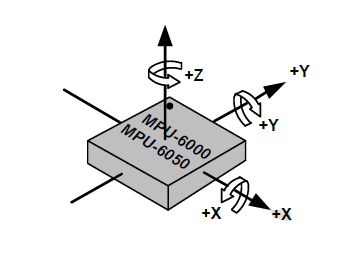
\includegraphics[scale=0.47]{Metodologia/IMUEixos}}
    \caption{A placa comercial é vista em (a) e os detalhes dos eixos do sensor de orientação utilizado para medição da inclinação do robô é visto em (b).}
    \label{fig:MPU6050}
\end{figure}

A partir do \textit{datasheet} da placa algumas características podem ser obtidas como visto na Tabela (\ref{tab:ParametrosPlacaMPU6050}).
\begin{table}[!htb]
\centering
\caption{Principais características da placa MPU6050 \citep{MPU6050}.}
\label{tab:ParametrosPlacaMPU6050}
\begin{tabular}{@{}lc@{}}
    \toprule
    \textbf{Descrição}              & \textbf{Valores}             \\ 
    \midrule
    Modelo                          & GY-521                        \\
    Tensão de Operação              & 3 $\sim$ 5 $V_{cc}$           \\
    Conversor ADC                   & 16 $bits$                     \\
    Comunicação                     & $I^2C$                        \\ 
    Tempo de Acomodação             & 10 $ms$                       \\
    Dimensões (C$\times$L$\times$A) & 21$\times$17$\times$3 $mm$    \\ 
    \bottomrule
\end{tabular}
\end{table}

\subsubsection{Acelerômetro}
O acelerômetro é um equipamento que é utilizado para mensurar sua aceleração própria. A aceleração própria é diferente daquela estabelecida através da relação entre velocidade e tempo. Sendo que esta considera a sensação de peso medida em um dado referencial. Quando considera-se o acelerômetro colocado em uma superfície plana, a medição será de aproximadamente $9.81 m/s^2$. Na maioria dos casos, a aceleração é medida em força g, que é basicamente a aceleração sentida como peso. A Figura (\ref{fig:InclinacaoAcelMPU}) mostra a inclinação de algum objeto utilizando dois eixos. 
\begin{figure}[H]
    \centering
    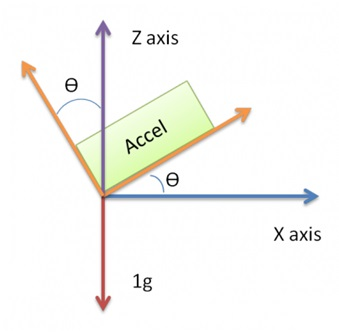
\includegraphics[scale=0.7]{Metodologia/Acelerometro}
    \caption{Detalhamento de forma gráfica dos 3 eixos do acelerômetro.}
    \label{fig:InclinacaoAcelMPU}
\end{figure}

A medição da orientação pode ser feita de três maneiras: utilizando apenas um eixo, dois e três eixos. A forma mais simples é a primeira, porém a mais eficiente em termos de precisão é a última. As equações são mostradas logo abaixo:
\begin{equation}
    \begin{array}{ccc}
         &  \theta = \sin^{-1}(x) \\[10pt]
         &  \theta = \arctan \left(\dfrac{x}{z}\right)  \\[10pt]
         &  \theta = \arctan \left(\dfrac{x}{\sqrt{z^2+y^2}}\right)
    \end{array}{}
\end{equation}{}

\subsubsection{Giroscópio}
O giroscópio por sua vez, é um dispositivo utilizado para manter ou medir a orientação. Um giroscópio mecânico normalmente consiste de um disco rotativo, em que os eixos ligados a ele são capazes de se deslocarem livremente em qualquer orientação. 

O valor lido da MPU6050 sem nenhum tratamento pode ser chamado de valor bruto já que não representa nenhuma grandeza física e para realizar a conversão para um valor usual, é necessário saber/configurar o quão rápido o sensor está girando em graus por segundo $(dps)$. A Tabela (\ref{tab:ParamGiroMPU}), com conteúdo encontrado no $\textit{datasheet}$ do fabricante, relaciona cada velocidade de giro do sensor com a sua sensibilidade, sendo que essas constantes são chamadas de ganho e devem ser divididas por 1000.
\begin{table}[!htb]
    \centering
    \caption{Parâmetros do giroscópio: velocidade de giro e nível de sensibilidade.}
    \label{tab:ParamGiroMPU}
    \begin{tabular}{@{}cc@{}}
        \toprule
        \textbf{Faixa ($^{\circ}$/s)} & \textbf{Sensibilidade LSB/($^{\circ}$/s)} \\ \midrule
        $\pm 250$                    & 131                                                   \\
        $\pm 500$                    & 65.5                                                  \\
        $\pm 1000$                   & 32.8                                                  \\
        $\pm 2000$                   & 16.4                                                  \\ \bottomrule
    \end{tabular}
\end{table}

\subsection{Bateria}

A escolha da bateria de Lipo de 2200mAh, como visto na Figura (\ref{fig:Bateria2200}), passou por alguns critérios, como o tempo de funcionamento e capacidade de fornecimento de energia. As características mais importantes encontradas no \textit{datasheet} do fabricante, é visto abaixo: 
\begin{table}[!htb]
    \centering
    \caption{Parâmetros do giroscópio: velocidade de giro e nível de sensibilidade.}
    \label{tab:ParamGiroMPU}
    \begin{tabular}{@{}lcc@{}}
        \toprule
        \textbf{Descrição} & \textbf{Valores} & \textbf{Unidade}              \\ 
        \midrule
        Tensão              & 7.4                       & $V_{cc}$     \\
        Capacidade          & 2.2                       & $Ah$         \\
        Descarga            & 30                        & $C$          \\
        Comprimento         & 105                       & $mm$         \\
        Largura             & 32                        & $mm$         \\
        Altura              & 16                        & $mm$         \\
        Massa               & 121.4                     & $g$          \\ 
        \bottomrule
    \end{tabular}
\end{table}

O item mais relevante a considerar é se a mesma consegue fornecer a capacidade necessária de energia para o sistema. O consumo máximo de corrente que a bateria pode fornecer é diretamente proporcional a sua capacidade ampére por hora ($Ah$) e sua taxa de carga e descarga, que nesse caso é de 30 $C$. O cálculo é simples e é realizado da seguinte forma
\begin{equation}\label{eq:CorrenteBateria}
    Corrente (A) = 2.2 Ah\times 20 C = 44 A
\end{equation}{}
assim, pela Equação (\ref{eq:CorrenteBateria}) a bateria vista na Figura (\ref{fig:Bateria2200}) suporta fornecer até 44A em teoria quando solicitada. Geralmente, se trabalha com uma margem de 50\% para preservá-la.
\begin{figure}[H]
    \centering
    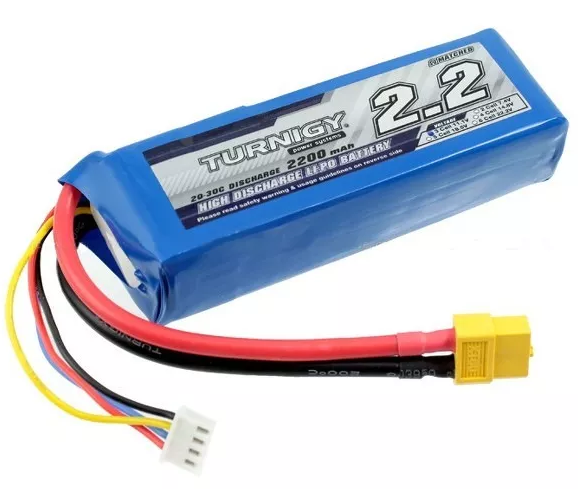
\includegraphics[scale=0.5]{Metodologia/Bateria2200}
    \caption{Bateria Lipo de duas células (7.4 $V_{cc}$) com capacidade de 2200 $mAh$ e taxa de carga e descarga 20 $C$.}
    \label{fig:Bateria2200}
\end{figure}

Com relação ao tempo de funcionamento, basta conhecer o valor de consumo de cada dispositivo que compõe o sistema. Para esse projeto, pode-se considerar apenas o consumo dos motores, Tabela (\ref{tab:ConsumoMotores}), já que a corrente drenada pelos outros eletrônicos são irrelevantes perante aos atuadores. Em teoria e considerando tudo em perfeitas condições, é possível obter 1 (uma) hora de funcionamento utilizando o torque máximo ou 110 min usando a máxima eficiência dos motores em descarga contínua. 
\begin{table}[!htb]
\centering
\caption{Consumo dos Motores CC.}
\label{tab:ConsumoMotores}
\begin{tabular}{@{}lcc@{}}
\toprule
\multicolumn{1}{c}{\textbf{Dispositivo}} & \textbf{Máx. Eficiência} & \textbf{Máx. Torque} \\ \midrule
Motores                          & 1.2 A                     & 2.2 A                 \\ \bottomrule
\end{tabular}
\end{table}

\subsection{Representação da Montagem do Circuito Eletrônico}

A representação esquemática do circuito eletrônico contendo todos os componentes detalhados aqui neste capítulo, pode ser visto na Figura (\ref{fig:circuitoEletronicoPlanta}). Pode-se observar através da figura como os componentes foram interligados uns aos outros. Essa é a representação final do circuito eletrônico para controle da posição angular da estrutura com a vertical.

\begin{figure}[H]
\centering
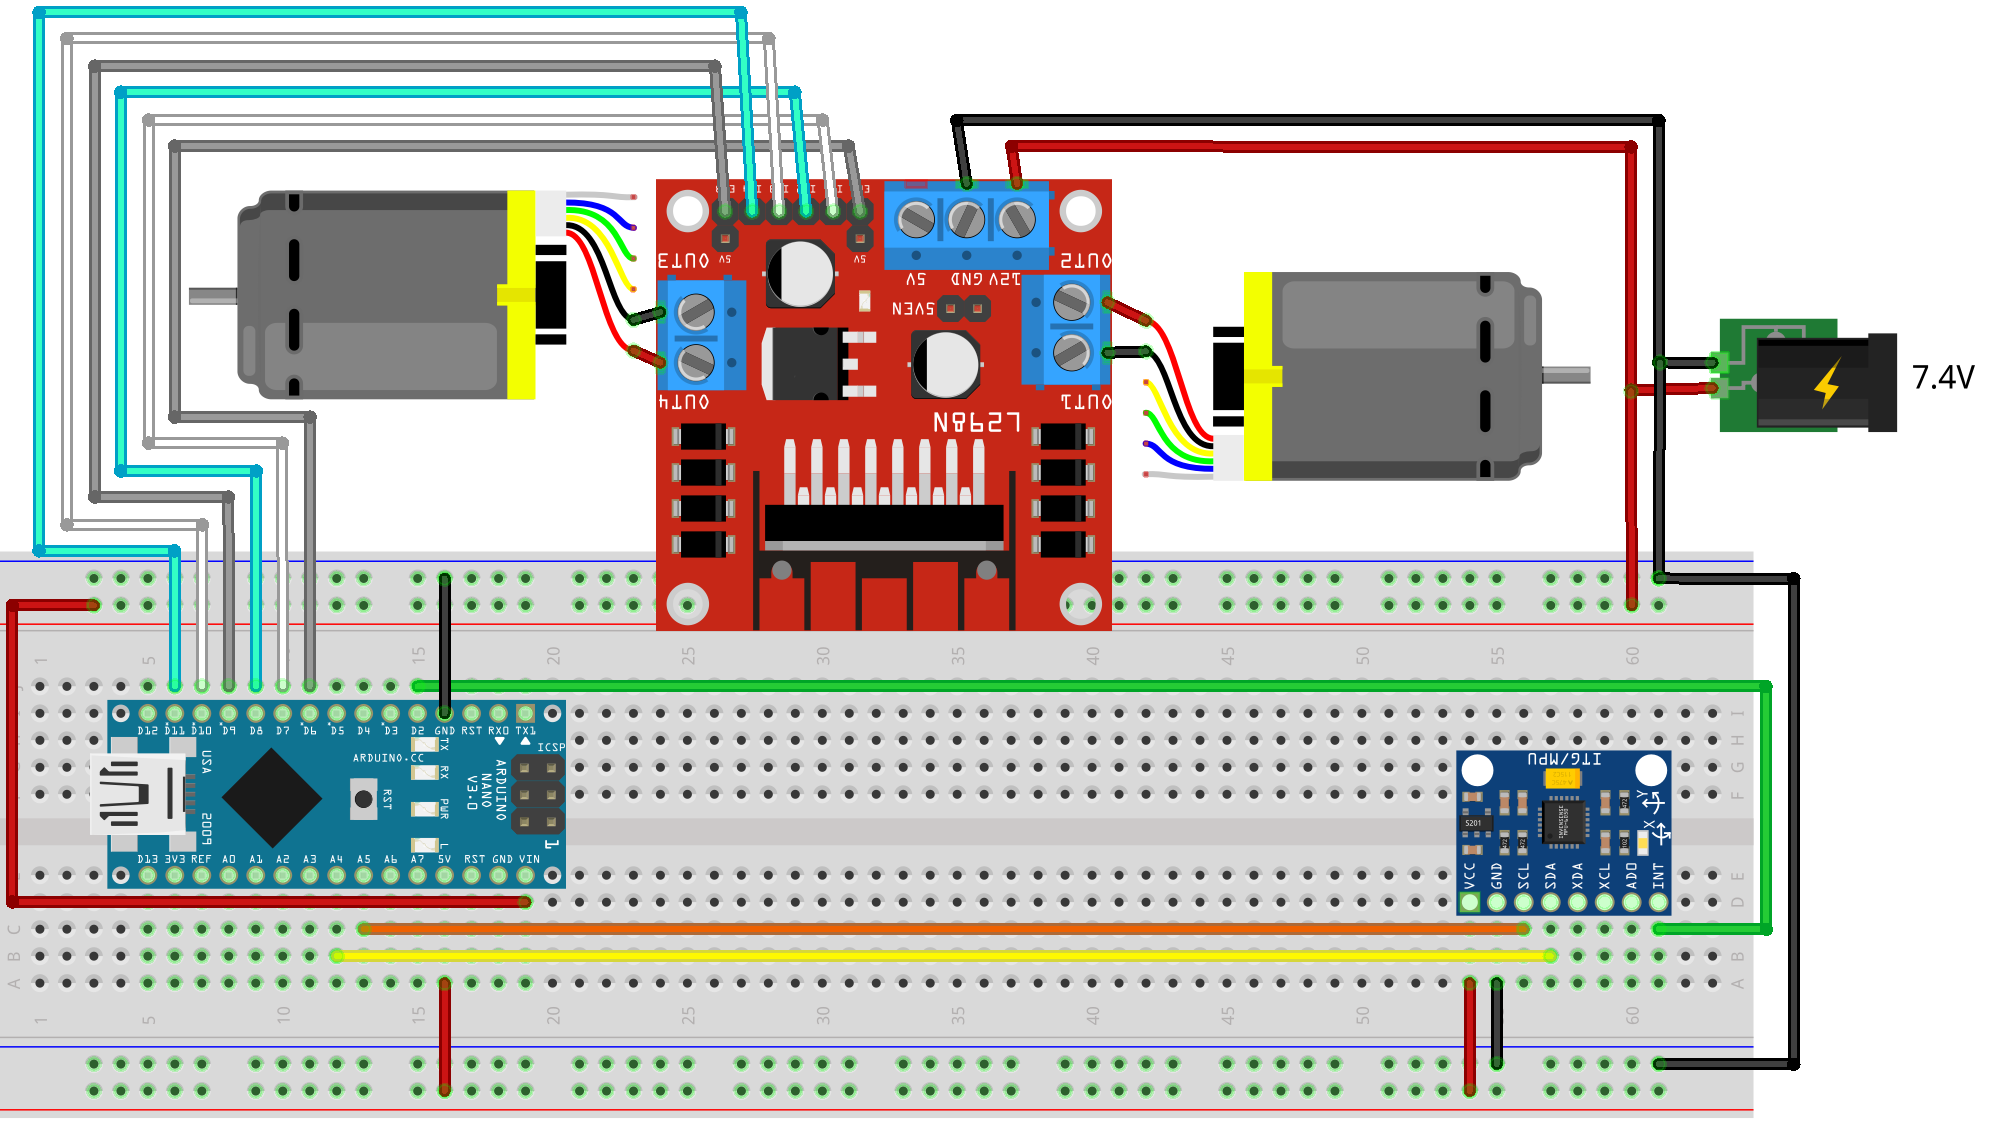
\includegraphics[width=16cm]{Resultados/CircuitoEletronico.png}
\caption{Representação do circuito eletrônico montado para controle da posição angular do pêndulo.}
\label{fig:circuitoEletronicoPlanta}
\end{figure}

\section{\textit{Softwares}}

A realização deste trabalho se deu através de uso de alguns \textit{softwares} que ajudaram e facilitaram bastante. Abaixo é feito um breve resumo de cada um e para qual propósito os mesmos serviram.

\subsection{SolidWorks}

O SolidWorks é um \textit{software} de CAD 3D, utilizado para modelagem de peças sólidas e para simulações de processos. Foi escolhido como plataforma para o desenvolvimento do projeto mecânico das peças da estrutura devido à experiência do autor com o programa, adquirido ao longo do curso.

\subsection{MATLAB}

O MATLAB é um \textit{software} interativo de alta performance voltado para o cálculo numérico. Realiza a análise numérica, cálculo com matrizes, processamento de sinais e construção de gráficos em ambiente fácil, sendo programado com linguagem matemática ao invés da programação tradicional. O \textit{software} conta com inúmeras extensões, mas com destaque para o Simulink. Essa extensão conta com uma programação baseada em diagrama de blocos e com esse \textit{toolbox} é possível realizar as simulações dos circuitos de uma forma que fique mais simples e de fácil visualização. Foi escolhido para realização dos cálculos de parâmetros mecânicos, dos ganhos do controlador e simulação do sistema.

\subsection{Arduino IDE}

É um \textit{software} gratuito, de código aberto, que facilita a gravação dos programas desenvolvidos na placa Arduino. A linguagem de programação é baseada em C. Foi utilizado no desenvolvimento do código responsável por acionar os motores de corrente contínua e também o processamento do controlador.

\subsection{Processing}

O Processing por sua vez é uma linguagem de programação de código aberto e possui um ambiente de desenvolvimento integrado (IDE). Contudo, ele é considerado um \textit{sketchbook}, alternativa de organização de projetos sem ser o de um IDE padrão. Por mais que seja baseado na linguagem Java, a forma de programar não é de Java puro, a não ser que o usuário deseja. Foi utilizado neste trabalho em conjunto com o Arduino para validação dos sinais do sensor, lendo dados através da porta serial do computador.

\subsection{Visual Studio Code (VS Code)}

O Visual Studio Code, ou popularmente conhecido como VS Code, é um editor de código-fonte desenvolvido pela Microsoft para Windows, Linux e macOS. É customizável, permitindo que os usuários possam mudar o tema do editor, teclas de atalho e preferências. É um \textit{software} livre e de código aberto. Foi utilizado para ler os sinais gravados em arquivo com extensão .txt do Processing utilizando linguagem python.

\subsection{\textit{Fritizing}}

O \textit{Fritizing} é uma iniciativa de código aberto para desenvolver um \textit{software} tipo CAD para desenhos de \textit{hardware} eletrônico, com intuito de apoiar a construção de um circuito mais permanente como a confecção de uma placa de circuito impresso (PCB). Utilizou desse \textit{software} para a elaboração de uma visão esquemática do circuito eletrônico da planta.

\section{Custo dos Materiais Adquiridos}

A seguir, na Tabela (\ref{tab:CustoMateriais}), estão listados os materiais utilizados para a elaboração mecânica e eletrônica do projeto, seus respectivos preços e a quantidade necessária.
\begin{table}[!htb]
\centering
\caption{Tabela de custo dos materiais utilizados na construção do protótipo.}
\label{tab:CustoMateriais}
\begin{tabular}{@{}lccccccc@{}}
\toprule
\multicolumn{1}{c}{\textbf{Descrição}} & \textbf{Un.} & \textbf{Qtd.} & \textbf{Valor Un.} & \textbf{Valor Total}  \\ \midrule
Arduino Nano            & pç  & 1   & R\$ 19,50   & R\$ 19,50   &                          \\
Kit Motor CC            & pç  & 2   & R\$ 119,90  & R\$ 239,80  &                          \\
Driver L298 H           & pç  & 1   & R\$ 19,90   & R\$ 19,90   &                          \\
MPU6050                 & pç  & 1   & R\$ 16,90   & R\$ 16,90   &                          \\
Bateria Lipo 2200mAh    & pç  & 1   & R\$ 130,00  & R\$ 130,00  &                          \\
Carregador Lipo Imax B6 & pç  & 1   & R\$ 110,00  & R\$ 110,00  &                          \\
Estrutura               & -   & 1   & R\$ 45,00   & R\$ 45,00   &                          \\
Miscelaneas             & -   & 1   & R\$ 58,00   & R\$ 58,00   &                           \\
\multicolumn{4}{l}{\textbf{TOTAL}}                                                       & \multicolumn{1}{l}{\textbf{R\$ 639,10}} \\ \bottomrule
\end{tabular}
\end{table}

O item denominado de miscelâneas da lista de materiais remete aos materiais que são difíceis de contar um a um e na maioria da vezes são parafusos, porcas, \textit{jumpers}, etc. Para encontrar seu valor, considerou-se 10\% do valor total de toda a lista.
\chapter{Modelagem do Sistema e Projeto do Controlador LQG}\label{cap:ModelagemProjetoControlador}

Este capítulo abordará a descrição do modelo matemático do pêndulo invertido sobre duas rodas. Para a obtenção das equações do modelo, utilizará de Euler-Lagrange para tal fim. O eixo é fixo no centro das rodas, sendo assim, o mesmo só move quando há movimento linear das rodas. O ângulo de inclinação do pêndulo é o $\theta$, que é a variável controlada, e a velocidade angular é $\dot{\theta}$.

\section{Modelagem do Motor de Corrente Contínua}\label{sec:ModeloEletricoMotor}

O circuito elétrico simplificado que modele os motores CC do projeto, pode ser visto na Figura (\ref{fig:M-motor}) \citep{Silva:17}. 
\begin{figure}[H]
	\centering
	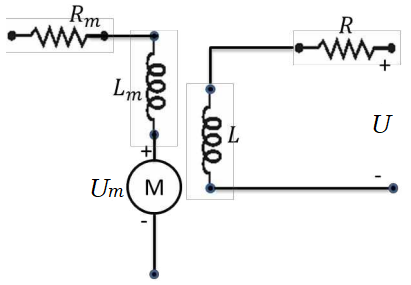
\includegraphics[scale=0.8]{Modelagem/Circuito_MotorDC.png}
	\caption{Representação esquemática do circuito elétrico do motor CC \citep{Silva:17}.}
	\label{fig:M-motor}
\end{figure}    

A variável $U$ representa a tensão de controle aplicada nos motores, $R$ e $L$ representam a resistência interna e a indutância dos enrolamentos do estator respectivamente. Aplicando a Lei das Tensões de Kirchoff (KVL), pode-se estabelecer uma relação entre as tensões internas do circuito dos motores CC considerando separadamente cada componente. Para o circuito da Figura (\ref{fig:M-motor}), obtém-se a seguinte equação.
\begin{gather}
	U = Ri + L\frac{di}{dt} + U_m\label{eq:eqEletricaMotor}
\end{gather}

Considerando a corrente elétrica do motor constante, desconsiderando reações na armadura, efeitos magnéticos secundários bem como deformidades na geometria do motor, o fluxo magnético que atravessa o entreferro do motor pode ser considerador constante e proporcional a velocidade angular do eixo do motor ($\dot{\varphi}$).
\begin{gather}
	U_m = k_e\dot{\varphi}\label{eq:eqConstanteEletricaMotor}
\end{gather}

A força resultante do eixo do motor é proporcional a corrente, ao número de espiras das bobinas entre outros fatores. O torque resultante que atua sobre o eixo é a multiplicação da força pelo raio dessas bobinas enroladas. Esses valores constantes que dependem da geometria e do material denomina-se de constante mecânica do motor ($k_m$) e o torque que é aplicado no eixo fica proporcional a corrente do motor CC, como mostra a Equação (\ref{eq:eqConstanteMecanicaMotor}).
\begin{gather}
	\tau_{m} = k_mi\label{eq:eqConstanteMecanicaMotor}
\end{gather}

Como o  sinal a ser controlado da planta será o da tensão, se faz necessário encontrar a expressão do torque em termos da mesma. Assim, o torque do motor em relação a tensão de entrada $U$ é vista na Equação (\ref{eq:eqTorqueMotor}) abaixo.
\begin{equation}\label{eq:eqTorqueMotor}
    \tau_{m} = \dfrac{k_{m}}{R}U - \dfrac{k_{m}k_{e}}{R}\dot{\varphi}_{eixo}
\end{equation}

Para encontrar as equações descritas acima, foram feitas várias simplificações. Um modelo mais fidedigno de um motor real consideraria várias não linearidades como por exemplo folgas mecânicas que aqui foram desconsiderados. 

Existe também uma outra propriedade muito importante de um motor que é a sua zona morta (dz- $\textit{dead zone}$). O conceito dessa propriedade é basicamente uma tensão abaixo da necessária que faça com que o eixo do motor entre em movimento, ou seja, é uma região de tensão entre o valor 0V e o valor mínimo de $\textit{input}$ que faça o motor girar.

\subsection{Estimando as Constantes Mecânica $k_m$ e Elétrica $k_e$ do Motor}

A partir dos dados fornecidos pelo fabricante, é possível encontrar as constantes mecânica $k_m$ e elétrica $k_e$ do motor. Com os dados que estão descritos na Tabela (\ref{tab:ParametrosDatasheetMotor}) e com a Equação (\ref{eq:eqTorqueMotor}) é possível estimar os valores utilizando a Equação (\ref{eq:eqTorqueMEstimarConstante}) abaixo.
\begin{equation}\label{eq:eqTorqueMEstimarConstante}
    \tau_{m} = \dfrac{k_{m}}{R}U - \dfrac{k_{m}k_{e}}{R}\dot{\varphi}_{eixo} = \alpha + \beta(\dot{\varphi}_{eixo})
\end{equation}

Realizando uma regressão linear com os dados fornecidos pelo fabricante, encontra-se para $\alpha$ e $\beta$ os seguintes valores: $\alpha$ = 0.99423 e $\beta$ = -0.04462.

De acordo com \cite{Silva:17}, para encontrar a constante elétrica $k_e$, considera-se que o torque seja praticamente nulo em velocidade máxima do eixo do motor. Dessa forma, o valor de $k_e$ pode ser calculado conforme a Equação (\ref{eq:eqCalculoConstanteKE}).
\begin{equation}\label{eq:eqCalculoConstanteKE}
    k_{e} = \dfrac{U}{\dot{\varphi}_{eixo}} = 0.2729
\end{equation}

Com a Equação (\ref{eq:eqConstanteMecanicaMotor}) e com os dados referente a torque vistos na Tabela (\ref{tab:ParametrosDatasheetMotor}), é possível se chegar em uma faixa de valores possíveis para a constante mecânica do motor $k_m$. Abaixo em (\ref{eq:eqCalculoConstanteKM}) é visto os valores encontrados para $k_m$.
\begin{equation}\label{eq:eqCalculoConstanteKM}
k_{m}(\tau_{m},i) =
\begin{cases}
    k_{eix.trav.} = \dfrac{\tau_{m}}{i} = 0.3065 \\[6pt]
    k_{max.efic.} = \dfrac{\tau_{m}}{i} = 0.3269 \\[6pt]
    k_{max.pot.}  = \dfrac{\tau_{m}}{i} = 0.4636
\end{cases}
\end{equation}

De forma a simplificar a escolha do valor de $k_m$ a ser utilizado no modelo, será realizado uma média ponderada, adotando os seguintes pesos: $P_{eix.trav.}$ = $1$, $P_{max.efic.}$ = $1$ e $P_{max.pot.}$ = $2$. Resolveu-se adotar um peso diferente para o $k_{max.pot.}$ já que seu valor está bem acima dos demais. Sendo assim, o valor final de $k_m$ é visto abaixo.
\begin{equation}\label{eq:eqCalculoConstanteKMFinal}
    k_{m} = \dfrac{0.3065 + 0.3269 + 2(0.4636)}{1 + 1 + 2} = 0.3902
\end{equation}

\section{Modelagem do Sistema baseada na Metodologia de Euler-Lagrange}\label{sec:EquaçõesMovimentoEstrutura}

Na Figura (\ref{fig:M-pendulo}) é mostrado o diagrama de corpo livre da parte estrutural do pêndulo invertido sobre duas rodas. Sendo que $z$ a distância que passa no eixo das rodas até o centro de massa representado por $CM$ e $\theta$ é a variável (ângulo entre o corpo e o eixo vertical) a ser controlada.
\begin{figure}[H]
		\centering
		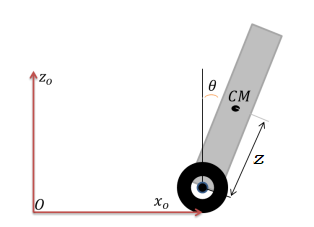
\includegraphics[scale=0.95]{Modelagem/RepresentacaoPendulo.png}
		\caption{Diagrama corpo livre do pêndulo invertido. Adaptado de \citep{Silva:17}.}
		\label{fig:M-pendulo}
\end{figure}  

Para a obtenção da modelagem, seguindo o princípio de Euler-Lagrange, é necessário determinar a energia cinética e a energia potencial total do conjunto formado pelo pêndulo e pelas rodas, conforme \cite{Faria:15}. A energia cinética total é dada pela soma das energias cinéticas lineares e rotacional do corpo do sistema e das rodas, como é mostrado por (\ref{eq:eqEnergiaCineticaFormula}) e (\ref{eq:eqEnergiaCineticaDescritiva}).
\begin{equation}\label{eq:eqEnergiaCineticaFormula}
    T = T_{\textit{r}}^{\textit{R}} + T_{\textit{p}}^{\textit{R}} + T_{\textit{r}}^{\textit{T}} + T_{\textit{p}}^{\textit{T}}
\end{equation}

\begin{equation}\label{eq:eqEnergiaCineticaDescritiva}
    T = \frac{1}{2}J_{r}\dot{\theta}^2 + \frac{1}{2}J_{p}\dot{\theta}^2 + \frac{1}{2}M_r\textit{v}_{r}^2 + \frac{1}{2}m_p\textit{v}_{p}^2
\end{equation}

As velocidades $\textit{v}_{r}$ e $\textit{v}_{p}$ representam, respectivamente as componentes de velocidades das rodas e do corpo do pêndulo. Os módulos de $\textit{v}_{r}$ e $\textit{v}_{p}$ são mostrados a seguir pelas Equações (\ref{eq:eqVelocidadeComponenteRoda}) e (\ref{eq:eqVelocidadeComponentePendulo}).
\begin{gather}
    v_r = \dot{x} = r\dot{\theta}
    \nonumber\\[1ex]
    |v_r|^2 = \dot{x}^2 = r^2\dot{\theta}^2\label{eq:eqVelocidadeComponenteRoda}
\end{gather}

\begin{gather}
    v_p =  \frac{d}{dt}(x + z_{cm}\sin{\theta}) + \frac{d}{dt}(z_{cm}\cos{\theta})
    \nonumber\\[1ex]
    |v_p|^2 = \left[\frac{d}{dt}(x + z_{cm}\sin{\theta})\right]^2  +  \left[\frac{d}{dt}(z_{cm}\cos{\theta})\right]^2 
    \nonumber\\[1ex]
    |v_p|^2 = \dot{x}^2 + 2z_{cm}\dot{x}\dot{\theta}\cos{\theta} + z_{cm}^2\dot{\theta}^2 \label{eq:eqVelocidadeComponentePendulo}
\end{gather}

Substituindo-se os valores encontrados nas equações (\ref{eq:eqVelocidadeComponenteRoda}) e (\ref{eq:eqVelocidadeComponentePendulo}) em (\ref{eq:eqEnergiaCineticaDescritiva}), determina-se a equação da energia cinética em função das posições e velocidades angulares, assim como mostra a Equação (\ref{eq:eqEnergiaCineticaPendulo}).
\begin{equation}\label{eq:eqEnergiaCineticaPendulo}
    T = \frac{1}{2}J_{eq}\dot{\theta}^2 + \frac{1}{2}m\dot{x}^2 + M_pz_{cm}\dot{x}\dot{\theta}\cos{\theta} + \frac{1}{2}M_pz_{cm}\dot{\theta}^2
\end{equation}

Sendo que $J_{eq}$ é equivalente a soma dos momentos de inércia do pêndulo $J_p$ e os das rodas $J_w$. No sistema temos uma única energia potencia $V$ que vem da gravidade e afeta somente o corpo do pêndulo. Essa energia é defina pela Equação (\ref{eq:eqEnergiaPotencialPendulo}).
\begin{equation}\label{eq:eqEnergiaPotencialPendulo}
    V = M_pgz_{cm}\cos{\theta}
\end{equation}

A equação de Lagrange de movimento para o PIDR é dada por (\ref{eq:eqEquacaoMovimentoLagrange}). Será trabalhado apenas com a equação de movimento para a variável de interessa $\theta$, uma vez que somente esta será possível de ser medida e controlada.
\begin{equation}\label{eq:eqEquacaoMovimentoLagrange}
    \frac{d}{dt}\left(\dfrac{\partial L}{\partial\dot{\theta}}\right) - \dfrac{\partial L}{\partial\theta} = \tau_{m}
\end{equation}

Nas equação descrita, o valor de $L$ é dado pela Equação (\ref{eq:eqEquacaoLagrange}), sendo $T$ e $V$ as energia cinética e potencial totais do pêndulo, respectivamente. O torque total aplicado ao pêndulo é representado pelo conjugado de saída $\tau_m$ do motor. 
\begin{equation}\label{eq:eqEquacaoLagrange}
    L = T - V
\end{equation}

Realizando a subtração da energia cinética e da energia potencial do sistema que foram determinadas, como mostrado em (\ref{eq:eqEquacaoLagrange}), encontra-se a equação para $L$. O resultado desta operação é dado por (\ref{eq:eqResultadoEquacaoLagrange}).
\begin{equation}\label{eq:eqResultadoEquacaoLagrange}
    L = \dfrac{1}{2}J_{eq}\dot{\theta}^2 + \dfrac{1}{2}m\dot{x}^2 + M_{p}z_{cm}\dot{x}\dot{\theta}\cos{\theta} + \dfrac{1}{2}M_{p}z_{cm}\dot{\theta}^2 - mgz_{cm}\cos{\theta}
\end{equation}

Como visto na Equação (\ref{eq:eqVelocidadeComponenteRoda}), há uma correspondência entre $\dot{x}$ e $\dot{\theta}$. Sendo assim, o resultado obtido em (\ref{eq:eqResultadoEquacaoLagrange}) que está em termos de duas variáveis, $x$ e $\theta$, será modificado para apenas a variável de interessa, $\theta$. O resultado é mostrado por (\ref{eq:eqResultadoEquacaoLagrangeTheta}).
\begin{equation}\label{eq:eqResultadoEquacaoLagrangeTheta}
    L = \dfrac{1}{2}J_{eq}\dot{\theta}^2 + \dfrac{1}{2}mr^2\dot{\theta}^2 + M_{p}z_{cm}r\dot{\theta}^2\cos{\theta} + \dfrac{1}{2}M_{p}z_{cm}\dot{\theta}^2 - mgz_{cm}\cos{\theta}
\end{equation}

Agora é possível voltar a equação de Lagrange de movimento para o pêndulo sobre duas rodas (\ref{eq:eqEquacaoMovimentoLagrange}), utilizando do resultado conseguido na Equação (\ref{eq:eqResultadoEquacaoLagrangeTheta}). Assim, por meio da Equação (\ref{eq:eqEquaçãoNaoLinearModelo}), obtém-se a equação não linear do sistema físico por meio de uma modelagem baseada em Euler-Lagrange.
\begin{equation}\label{eq:eqEquaçãoNaoLinearModelo}
    (J_{eq} + mr^2 + 2M_{p}z_{cm}r\cos{\theta} + M_{p}z_{cm})\ddot{\theta} - (M_{p}z_{cm}r\sin{\theta})\dot{\theta}^2 - mgz_{cm}\sin{\theta } = \tau_{m}
\end{equation}

O torque de saída do motor $\tau_{m}$ em termos da tensão elétrica é definido pela Equação (\ref{eq:eqTorqueMotor}), na qual a variável $U$ corresponde à tensão elétrica de entrada controlada. A Equação (\ref{eq:eqTorqueMotorFinal}) define a equação final do torque do motor para o modelo deste trabalho, na qual considera-se que a velocidade angular do eixo do motor $\dot{\varphi}$ corresponde a velocidade angular do corpo do pêndulo $\dot{\theta}$ como forma de aproximação, já que esta é a única variável a ser medida.
\begin{equation}\label{eq:eqTorqueMotorFinal}
    \tau_{m} = \dfrac{k_{m}}{R}U - \dfrac{k_{m}k_{e}}{R}\dot{\theta}
\end{equation}

Por fim, para a realização da linearização por matrizes Jacobianas conforme descrito na seção (\ref{sec:Linearizacao}), considera-se que $\dot{x_{2}}$ = $\ddot{\theta}$, $\dot{x_{1}}$ = $x_{2}$ = $\dot{\theta}$, $x_{1}$ = $\theta$ e $u$ = $U$. Dessa forma, temos as seguintes equação de movimento não linear que descreve o sistema físico
\begin{equation}
f_{i}(x,u) =
\begin{cases}
    \dot{x_{1}} = x_{2} = \dot{\theta} \\[6pt]
    \dot{x_{2}} = \ddot{\theta} = \dfrac{(K_{m}u - K_{e}x_{2}) + (M_{p}z_{cm}r\sin{x_{1}})x_{2}^2 + mgz_{cm}\sin{x_{1}}}{J_{eq} + mr^2 + M_{p}z_{cm}(1 + 2r\cos{x_{1}})}
\end{cases}
\end{equation}
sendo $K_{m}$ = $\dfrac{k_{m}}{R}$ e $K_{e}$ = $\dfrac{k_{m}k_{e}}{R}$. 
\newline

Para linearizar as equações encontradas, é preciso escolher um ponto de equilíbrio desejado. Sendo assim, escolheu-se o seguinte valor: $x_{1}^{eq}$ = $x_{2}^{eq}$ = $u^{eq}$ = 0. O resultado da linearização conforme visto em (\ref{eq:MatrizesLineares}) é mostrado na Equação (\ref{eq:EquaçõesLinearizadasPorJacobiano})

\begin{equation}\label{eq:EquaçõesLinearizadasPorJacobiano}
    \begin{array}{cc}
         &  \dfrac{\partial f_{1}(x^{eq},u^{eq})}{\partial x_{1}} = 0 ~~~~~~~~~~~        \dfrac{\partial f_{1}(x^{eq},u^{eq})}{\partial x_{2}} = 1 \\\\
             
         &  \dfrac{\partial f_{2}(x^{eq},u^{eq})}{\partial x_{1}} =    \dfrac{mgz_{cm}}{\rho} ~~~~~~~~
            \dfrac{\partial f_{2}(x^{eq},u^{eq})}{\partial x_{2}} = \dfrac{-K_{e}}{\rho} \\\\
        
        &   \dfrac{\partial f_{1}(x^{eq},u^{eq})}{\partial     u} = 0 ~~~~~~~~~~~~~~
            \dfrac{\partial f_{2}(x^{eq},u^{eq})}{\partial     u} = \dfrac{K_m}{\rho}
    \end{array}{}
\end{equation}
sendo que $\rho$ = $J_{eq} + mr^2 + M_{p}z_{cm}(1 + 2r)$.

Feito isso, é possível definir as matrizes $A$, $B$, $C$ e $D$ do modelo linearizado. Essas matrizes são mostradas logo abaixo.
\begin{equation*}
A = \begin{bmatrix}
        0 & 1 \\\\
        \dfrac{mgz_{cm}}{J_{eq} + mr^2 + M_{p}z_{cm}(1 + 2r)} & \dfrac{-k_{m}k_{e}}{R(J_{eq} + mr^2 + M_{p}z_{cm}(1 + 2r))}
    \end{bmatrix}
\end{equation*}

\begin{equation*}
B = \begin{bmatrix}
        0 \\\\
        \dfrac{k_{m}}{R(J_{eq} + mr^2 + M_{p}z_{cm}(1 + 2r))}
    \end{bmatrix}
\end{equation*}

\begin{equation*}
C = \begin{bmatrix}
        1 & 0
    \end{bmatrix}
\end{equation*}

\begin{equation*}
D = \begin{bmatrix}
        0
    \end{bmatrix}
\end{equation*}

\section{Projeto do Controlador de Estabilização}

O controlador que será projetado nesta seção tem a função de estabilizar e manter o pêndulo na posição de equilíbrio instável e não natural, ou seja, esse controlador busca manter o corpo do pêndulo em $\theta$ = 0$^\circ$. Assim como explicado e mostrado em capítulos anteriores, o controlador atuará apenas em uma estreita faixa, a mais próxima do ponto desejada, uma vez que a linearização ocorreu em torno do ponto de equilíbrio.

Na literatura, há uma variada coleção de métodos que podem ser implementados com intuito de definir parâmetros de estratégias de controle. O método \textit{``Linear Quadratic Regulator" (LQR)} em conjunto com o \textit{``Linear Quadratic Estimator" (LQE)} formam o \textit{``Linear Quadratic Gaussian" (LQG)} que é uma técnica robusta e apropriada para encontrar os parâmetros de equilíbrio do sistema. Dado que as equações de movimento do sistema podem ser descritas na forma de espaço de estados, conforme a Equação (\ref{eq:SSContinuo}).

Na seção (\ref{sec:MetodologiaControladorLQG}) é explicado como funciona e o que é necessário realizar para se obter os parâmetros do controlador \textit{LQG}. O algoritmo do \textit{LQR} calcula uma ação de controle $u$ para minimizar a função custo $J$ como mostrado pela Equação (\ref{eq:eqFuncaoCustoCasoContinuo})
\begin{equation}\label{eq:eqFuncaoCustoCasoContinuo}
    J = \int_{0}^{\infty} x(t)^TQx(t) + u(t)^TRu(t)dt
\end{equation}
sendo que as matrizes $Q$ e $R$ definem o peso do vetor de estado e o peso sobre a ação de controle. Percebe-se que se $Q$ for aumentado, o controlador deve trabalhar mais para minimizar o custo da função e consequentemente, o ganho do controle resultante será maior. O vetor de estado do nosso sistema é definido como sendo:
\begin{equation*}
x = \begin{bmatrix}
        \theta & \dot{\theta}
    \end{bmatrix} ^ T
\end{equation*}

Por sua vez, a matriz $R$ será um escalar uma vez que estamos trabalhando em um sistema SISO. Sendo assim, o único sinal de entrada que a planta terá será a tensão de alimentação do motor $U$.

\subsection{Controlador LQR}\label{subsec:ResultadoControladorLQR}

Na seção (\ref{sec:MetodologiaControladorLQG}) foram descritos os procedimentos necessários para se determinar os ganhos de realimentação de estados. Para a realização do cálculo deste ganho utilizou-se o pacote $\textit{MathWorks}$ do $\textit{software}$ principal utilizado neste trabalho, o $\textit{MATLAB}$.  %^{\tiny{\circledR}}

Com os valores dos ganhos definidos pelo projeto, os pólos desejados para o sistema realimentado são obtidos. De forma a mostrar e provar que o sistema é realmente instável, mostra-se primeiramente os pólos de malha aberta. Assim, fica claro e simples de verificar a instabilidade do sistema em espaço de estados, obtido com a linearização exibida na seção (\ref{sec:EquaçõesMovimentoEstrutura}). A Figura (\ref{fig:Circulo-Unitario-Discreto}) mostra o mapa de pólos e zeros para o sistema em malha aberta.
\begin{figure}[H]
    \centering
    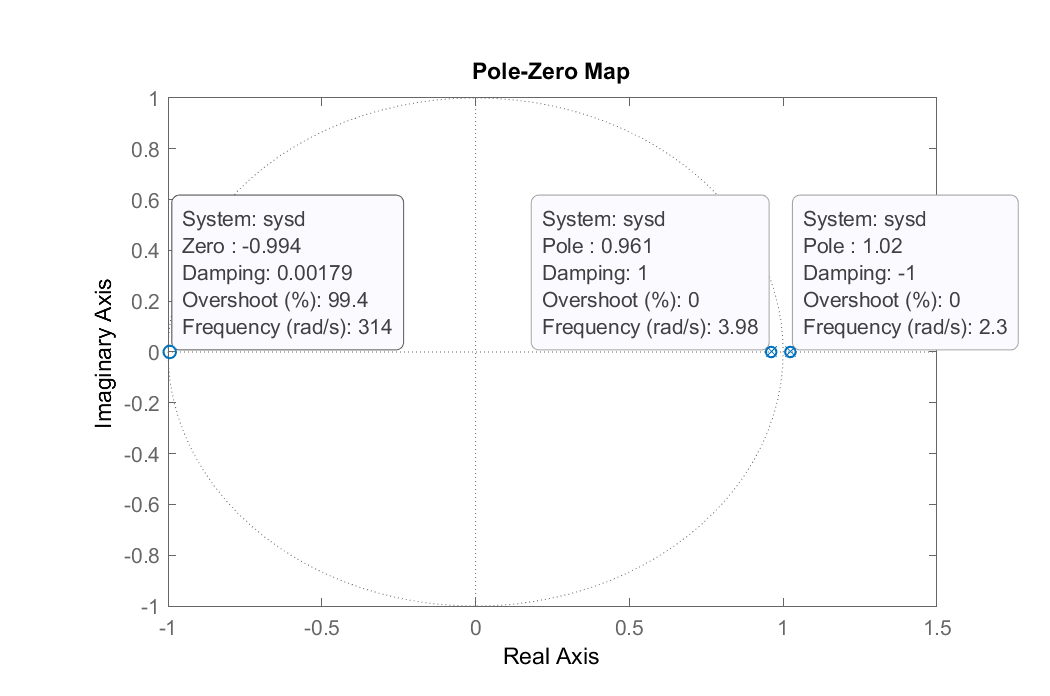
\includegraphics[scale=0.7]{ProjControladores/pzmap_discreto.eps}
    \caption{Círculo unitário de pólos e zeros do modelo discretizado.}
    \label{fig:Circulo-Unitario-Discreto}
\end{figure}{}

Ao analisar a Figura (\ref{fig:Circulo-Unitario-Discreto})), identifica-se um zero em $-0.994$ e os autovalores de malha aberta do sistema discreto como
\begin{equation*}
\lambda_{MA} = \begin{bmatrix}
        0.9610 & 1.0232
    \end{bmatrix}
\end{equation*}
sendo que pólo que mais a direita e fora do círculo unitário, confirma a instabilidade do sistema, de acordo com a literatura. Sendo assim, o controlador deverá levar este pólo para dentro do círculo unitário, ou seja, para dentro da região de estabilidade.

Utilizando-se da função $dlqr$ do $MATLAB$, o ganho $K_{lqr}$ do controlador é encontrado. A utilização deste comando depende das matrizes do espaço de estados do sistema discretizado pelo período de amostragem $T_s$ = $0.01 s$ escolhido - $A$, $B$, $C$ e $D$ - e dos pesos das matrizes da função de custo - $R$ e $Q$. A obtenção dos pólos de malha fechada desejados é obtido ao calcular o ganho do controlador com a função $dlqr$ ou fazendo $(A-BK_{lqr})$. Em relação aos pesos das matrizes da função de custo, definiu-se pesos unitários de modo a conseguir um controlador ótimo entre o custo sobre a ação e a precisão de controle. Abaixo em (\ref{eq:VetorGanhoLQR}) e (\ref{eq:AutovaloresSistemaRealimentadoLQR}), é o mostrado o vetor de ganho $K_{lqr}$ do controlador e o vetor dos pólos de malha fechada $\lambda_{MF}$.
\begin{equation}\label{eq:VetorGanhoLQR}
K_{lqr} = 
        \begin{bmatrix}
            k_{\theta} & k_{\dot{\theta}}
        \end{bmatrix} =
        \begin{bmatrix}
            3.2023 & 1.1508
        \end{bmatrix}
\end{equation}\label{eq:AutovaloresSistemaRealimentadoLQR}
\begin{equation}
\lambda_{MF} = \begin{bmatrix}
        0.9855 & 0.9272
    \end{bmatrix}
\end{equation}

Com intuito de visualizar de forma gráfica o comportamento do modelo não linear com o controlador projetado, elaborou-se uma simulação na plataforma $Simulink$ do $MATLAB$. Sabendo-se que a linearização ocorreu em uma região em torno do equilíbrio que é de $\theta$ = $0^\circ$, setou como condições iniciais para o modelo $\theta_0$ = $5^\circ$ e $\dot{\theta}_0$ = $0^\circ/s$. A Figura (\ref{fig:Implementacao-LQR}) mostra o conjunto de blocos necessários para a implementação do regulador no $Simulink$. 
\begin{figure}[H]
    \centering
    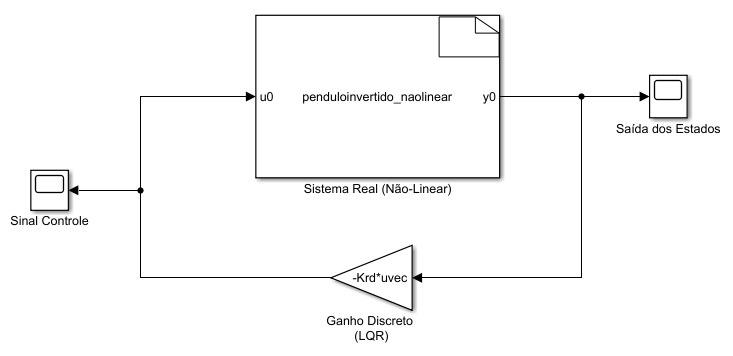
\includegraphics[scale=0.7]{ProjControladores/lqr_control.png}
    \caption{Modelo não linear realimentado pelo controlador $LQR$.}
    \label{fig:Implementacao-LQR}
\end{figure}{}

As seguintes Figuras (\ref{fig:RespostaEstados-LQR}) e (\ref{fig:SinalControle-LQR}) são as respostas dos estados e o sinal de controle respectivamente para o sistema realimentado apenas com o regulador e sem um observador de estados.
\begin{figure}[H]
    \centering
    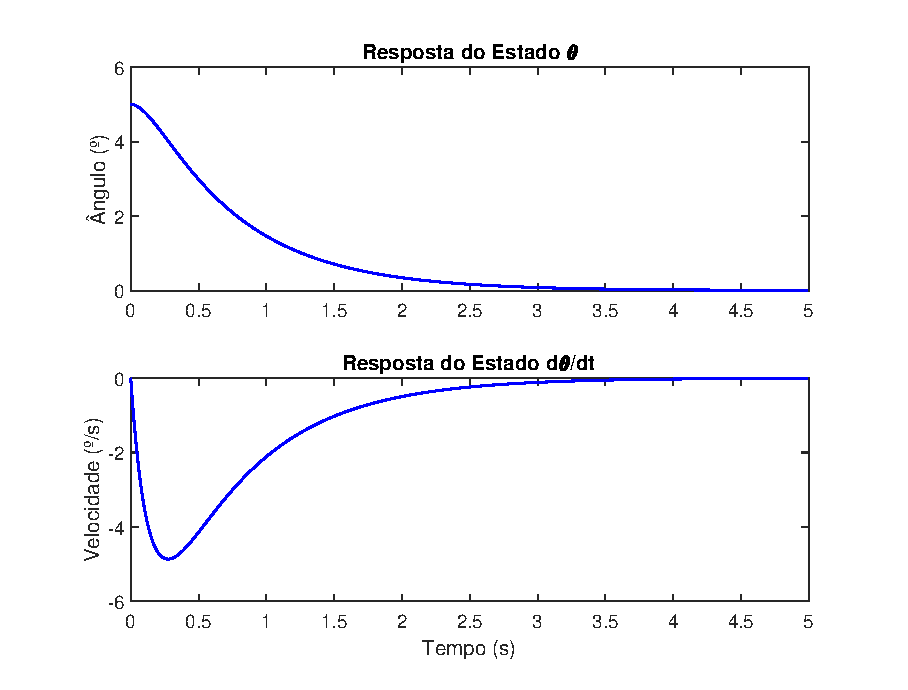
\includegraphics[scale=0.75]{ProjControladores/lqr_estados.eps}
    \caption{Respostas dos estados do sistema para a condição inicial estabelecida.}
    \label{fig:RespostaEstados-LQR}
\end{figure}{}
\begin{figure}[H]
    \centering
    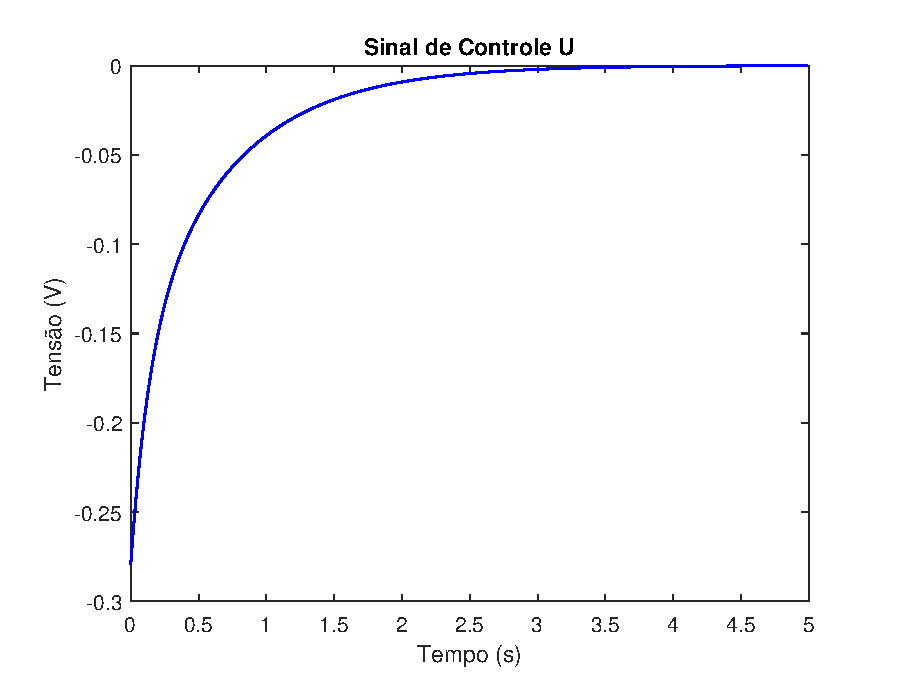
\includegraphics[scale=0.75]{ProjControladores/lqr_sinal_controle.eps}
    \caption{Sinal de controle do sistema para a condição inicial estabelecida.}
    \label{fig:SinalControle-LQR}
\end{figure}{}


\subsection{Estimador de Estados (Filtro de Kalman)}

A subseção (\ref{subsec:ResultadoControladorLQR}) deixa claro que com apenas o ganho do controlador $LQR$, temos um resultado satisfatório. Contudo, o intuito do deste trabalho é realizar o projeto de um estimador de estados para que o mesmo consiga melhorar significativamente o sinal de saída dos mesmos. Quando realizamos a junção tanto do $LQR$ quanto de um estimador de estados, obtemos o $LQG$ que tende a ser mais robusto e menos sensível a ruídos de medição e distúrbios. A simulação do sistema que agora contém um observador de estados, foi realizada sob as mesmas condições da simulação anterior. Sendo assim, as condições iniciais inseridas foram $\theta_0$ = $5^\circ$ e $\dot{\theta}_0$ = $0^\circ/s$. O \textit{design} do sistema com o acréscimo do $LQE$ é visto nas Figuras (\ref{fig:Implementacao-LQG}) e (\ref{fig:Topografia-controladorLQG}).
\begin{figure}[H]
    \centering
    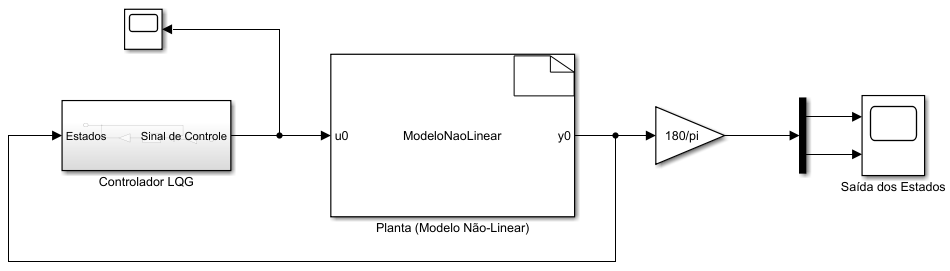
\includegraphics[scale=0.6]{ProjControladores/lqg_control.png}
    \caption{Modelo não linear realimentado pelo controlador $LQG$.}
    \label{fig:Implementacao-LQG}
\end{figure}{}
\begin{figure}[H]
    \centering
    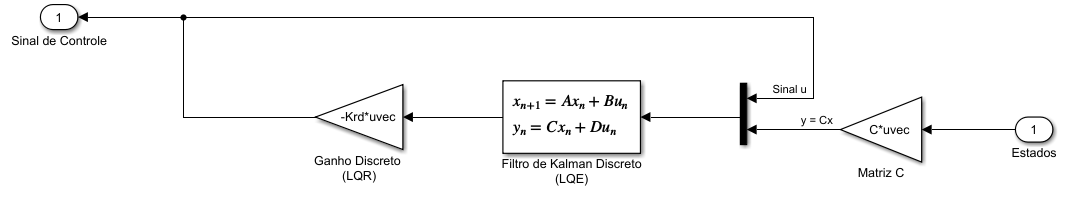
\includegraphics[scale=0.5]{ProjControladores/topografia_lqg.png}
    \caption{Detalhamento do controlador $LQG$.}
    \label{fig:Topografia-controladorLQG}
\end{figure}{}

Com essa nova topografia, realizamos o mesmo teste realizado anteriormente no qual a planta tinha apenas o regulador. As condições iniciais para a planta são as mesmas como já mencionado, o que difere agora são as condições iniciais do observador que foram setadas como sendo $\hat{\theta}$ = $\dot{\hat{\theta}}$ = $0$. Abaixo, nas Figuras (\ref{fig:RespostaEstados-LQG}) e (\ref{fig:SinalControle-LQG}) é visto a resposta dos sinais dos estados e do sinal de controle respectivamente.

\begin{figure}[H]
    \centering
    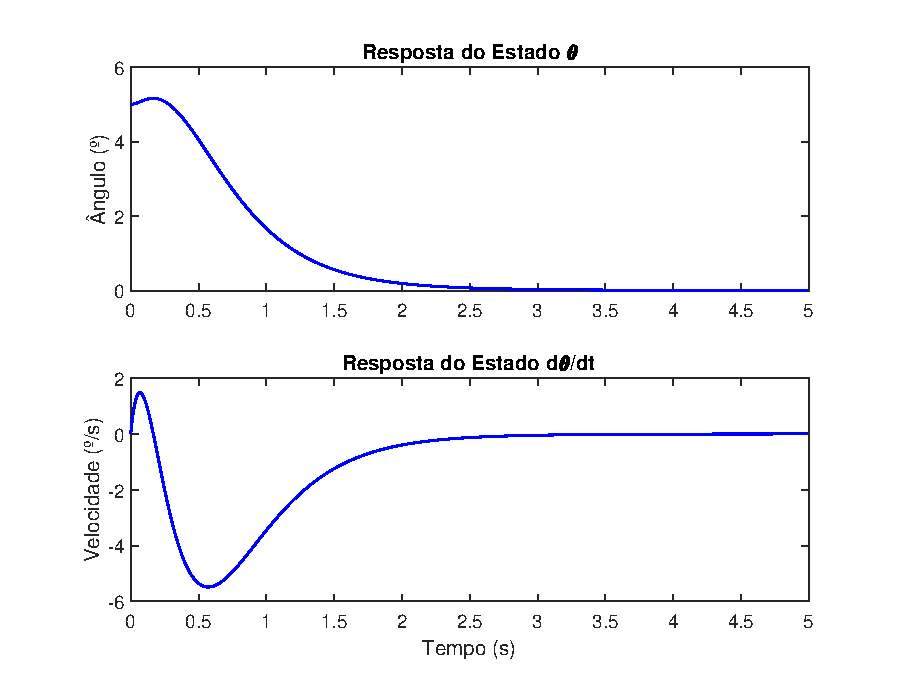
\includegraphics[scale=0.75]{ProjControladores/lqg_estados.eps}
    \caption{Respostas dos estados do sistema para a condição inicial estabelecida.}
    \label{fig:RespostaEstados-LQG}
\end{figure}{}

\begin{figure}[H]
    \centering
    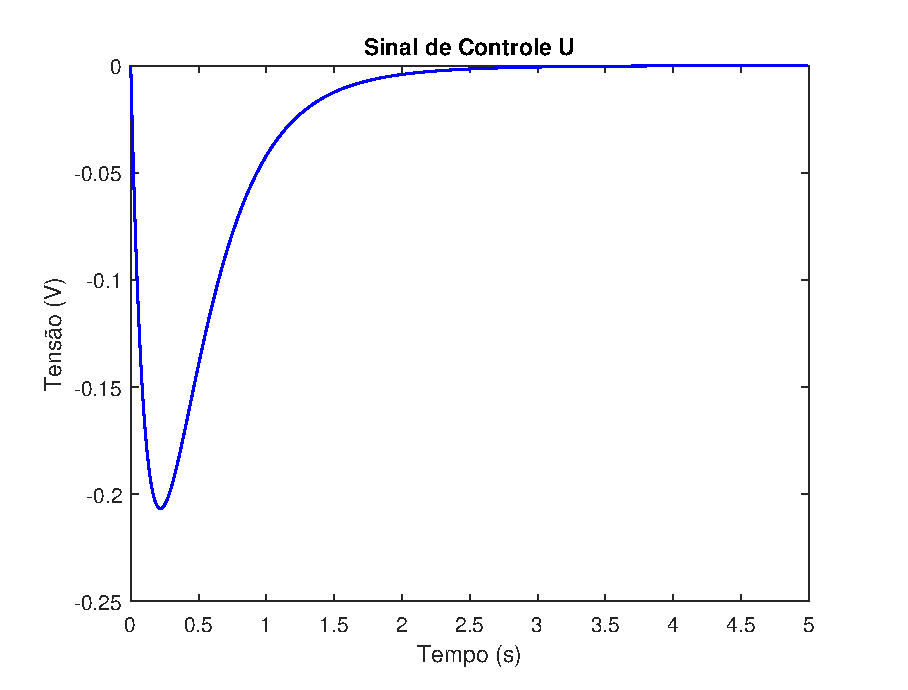
\includegraphics[scale=0.75]{ProjControladores/lqg_sinal_controle.eps}
    \caption{Sinal de controle do sistema para a condição inicial estabelecida.}
    \label{fig:SinalControle-LQG}
\end{figure}{}


\subsubsection{Inserção de Distúrbio e Ruído de Medição ao Sistema}

Como visto, em condições ideais e não reais já que todo sinal de medição haverá algum tipo de ruído, distúrbio e outras perturbações que está sendo até simplificado já no modelo, percebe-se que o controlador atua muito bem e sem dificuldade para estabilizar a planta. Dessa maneira, para testar o modelo de forma mais real e obter um resultado mais fidedigno do que realmente irá acontecer ao embarcar o controlador na planta física, resolveu-se incorporar ao sistema um sinal de ruído branco na resposta do sensor. Esse sinal, como visto na Figura (\ref{fig:SinalRuidoBranco}), possui um \textit{range} $\pm 1^\circ$, ou seja, quer dizer o sensor pode estar errando tanto $1^\circ$ positivo quanto $1^\circ$ negativo.
\begin{figure}[H]
    \centering
    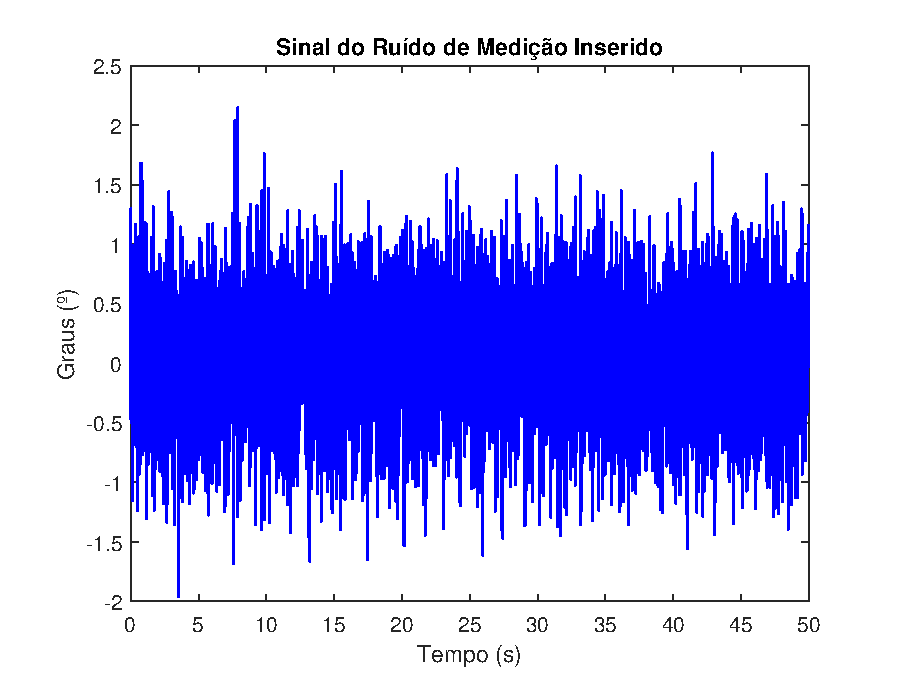
\includegraphics[scale=0.75]{ProjControladores/ruido_branco_medicao.eps}
    \caption{Sinal do ruído branco de medição.}
    \label{fig:SinalRuidoBranco}
\end{figure}{}

Além do ruído inserido, também decidiu-se por aplicar um distúrbio na simulação com intuito de visualizar o comportamento do controlador perante a uma adversidade, uma vez que após um certo tempo de início o sistema tende a ficar estável. Sendo assim, de forma proposital aplicou um sinal quadrático de duração de 0.5$s$, iniciando em t = 20$s$ e com amplitude de $3^\circ$. O \textit{design} do sistema com essas novas dificuldades impostas ao controlador é visto na Figura (\ref{fig:Implementacao-LQG-real}).
\begin{figure}[H]
    \centering
    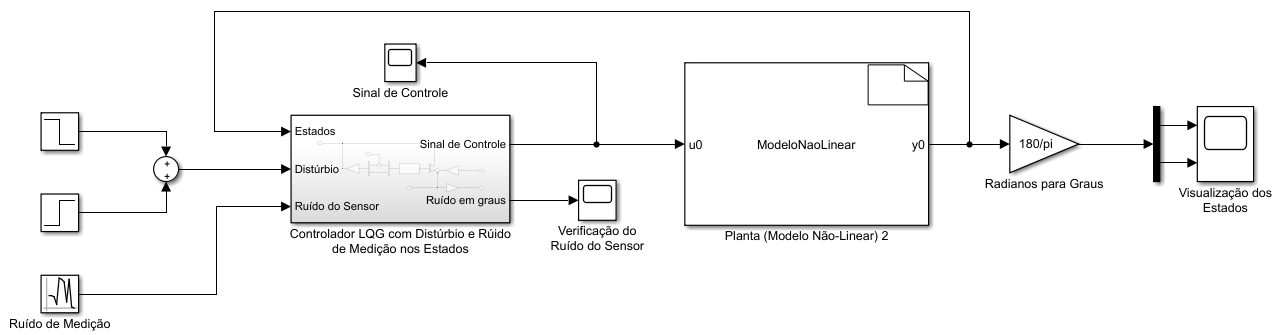
\includegraphics[scale=0.5]{ProjControladores/lqg_control_real.png}
    \caption{Modelo não linear realimentado pelo controlador $LQG$ com inserção de distúrbio e ruídos.}
    \label{fig:Implementacao-LQG-real}
\end{figure}{}

A Figura (\ref{fig:Topografia-controladorLQG-real}) mostra o detalhamento do controlador $LQG$ com o distúrbio e o ruído aplicado. Como é visto, o sinal do sinal do distúrbio é somado juntamente ao estado $\hat{\theta}$, antes de passar pelo regulador. Por sua vez, o sinal de ruído é somado ao sinal de medição realimentado.
\begin{figure}[H]
    \centering
    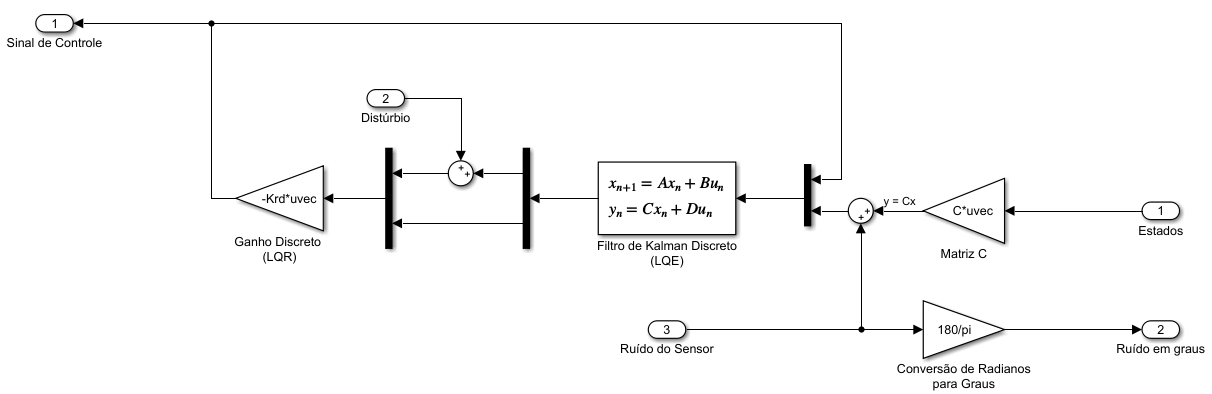
\includegraphics[scale=0.5]{ProjControladores/topografia_lqg_real.png}
    \caption{Detalhamento do controlador $LQG$ com a inserção de distúrbio e ruído de medição.}
    \label{fig:Topografia-controladorLQG-real}
\end{figure}{}

Contudo, para aproximar mais da realidade é inserido ao sistema um sinal quadrático de duração de 0.5$s$, iniciando em t = 20$s$ e com amplitude de $3^\circ$.

\begin{figure}[H]
    \centering
    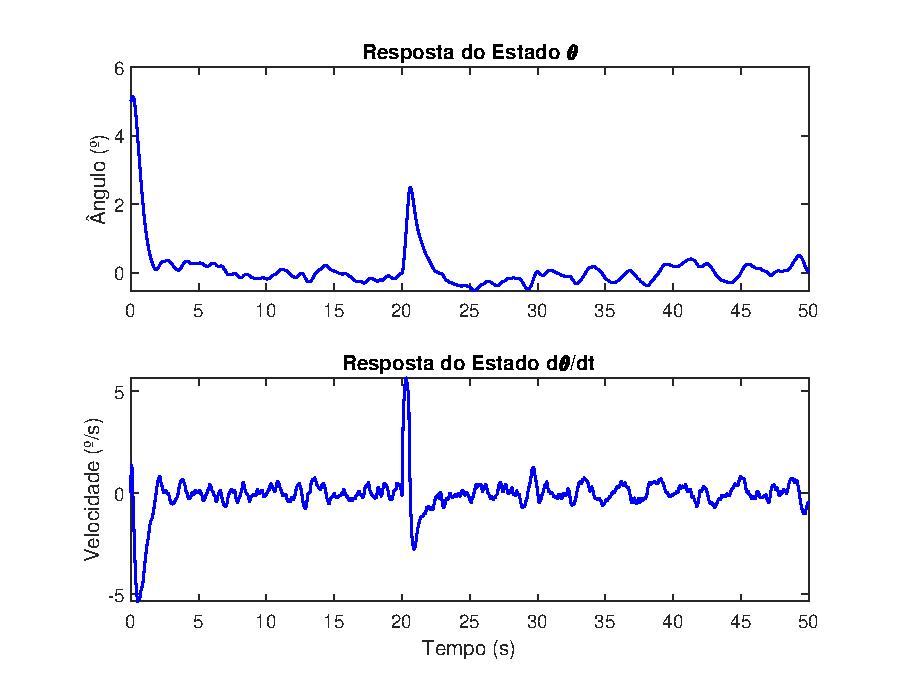
\includegraphics[scale=0.75]{ProjControladores/lqg_real_estados.eps}
    \caption{Respostas dos estados do sistema para a condição inicial estabelecida.}
    \label{fig:RespostaEstados-LQG-real}
\end{figure}{}

\begin{figure}[H]
    \centering
    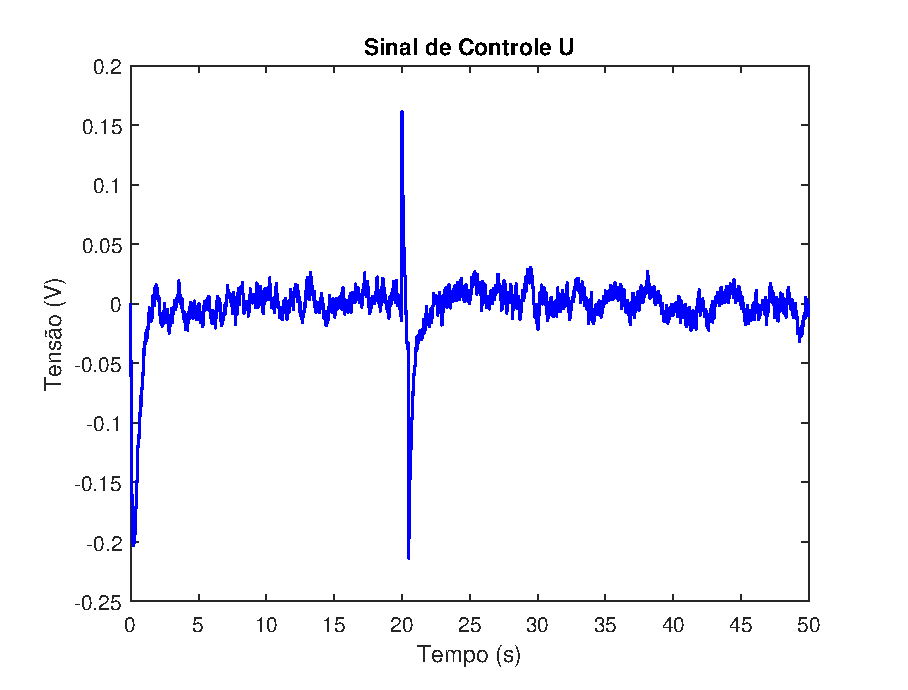
\includegraphics[scale=0.75]{ProjControladores/lqg_real_sinal_controle.eps}
    \caption{Sinal de controle do sistema para a condição inicial estabelecida.}
    \label{fig:SinalControle-LQG-real}
\end{figure}{}




\chapter{Resultados Práticos}

Este capítulo abordará os resultados práticos obtidos durante o desenvolvimento deste trabalho.

\section{Montagem da Planta}

Como relatado na Seção \ref{sec:EstruturaCAD}, ao se desenhar as placas da estrutura em \textit{software} CAD levou-se em consideração os furos para os componentes e passagem das cablagens. Em relação ao material, as mesmas são de ACM preto e foram cortadas por uma fresadora para um melhor acabamento e precisão. A Figura (\ref{fig:vistasMontagemPlanta}) mostra duas vistas da montagem, frontal e lateral. Além da estrutura mecânica, é visto também o conjunto de motores e rodas e os componentes eletrônicos.

\begin{figure}[H]
\centering
\includegraphics[width=8cm]{Resultados/MontagemFrontal.png}
\includegraphics[width=8cm]{Resultados/MontagemLateral.png}
\caption{Vistas frontal e lateral da montagem da planta física.}
\label{fig:vistasMontagemPlanta} 
\end{figure}

\section{Validação do Sensor e Motores}

Com a finalização da construção da planta física, projeto do controlador e realização da simulação conforme mostrado no Capítulo \ref{cap:ModelagemProjetoControlador}, foram realizados testes práticos para verificação do funcionamento do sistema montado. Foi desenvolvido um código utilizando a linguagem C, uma vez que a placa controladora será o microcontrolador Arduino. Essa placa tem como principal responsabilidade o processamento do sinal do sensor de posição angular para obtenção do sinal de controle utilizando dos ganhos do controlador LQG e consequentemente, gerando um sinal PWM para a placa L298N acionar os motores de corrente contínua. O código desenvolvido está em meu \href{https://github.com/mferreiracosta/tcc_cefet.git}{github}, mas a ideia de funcionamento é, basicamente:

\begin{itemize}
    \item se a estrutura tender a ir para frente, os motores receberão um valor de PWM e um comando para ir para frente. O valor do PWM é dependente de uma multiplicação matricial do valor do sinal do sensor filtrado e do ganho do regulador linear quadrático.
    \item caso a estrutura for para trás, o comando que a placa L298N receberá será contrário aquele recebido quando a estrutura for para frente. A lógica cálculo do valor do PWM se mantém a mesma.
\end{itemize}

Após desenvolvimento do código, esse foi carregado para o Arduino para obtenção dos sinais do sensor e acionamento dos motores para testes de movimentação. O circuito eletrônico montado tanto para testes quanto para controle da posição do pêndulo está esquematizado na Figura (\ref{fig:circuitoEletronicoPlanta}). Os resultados são visto abaixo.

\subsection{Validação do Sensor}

Após a montagem do circuito eletrônico, como mostrado acima na Figura (\ref{fig:circuitoEletronicoPlanta}), desenvolvimento do código Arduino e carregamento do mesmo na placa, foi possível realizar as validações. Primeiramente, focou-se em validar os sinais do sensor. A ideia é ver a diferença entre o sinal real do sensor e o filtrado por Kalman, afim de corroborar com o que a literatura afirma a respeito deste filtro, de que o mesmo traz uma maior robustez e é menos sensível a ruídos e distúrbios.

Entretanto, para obter os dados do sensor só foi possível através da serial da porta do computador, uma vez que neste trabalho não se utiliza de nenhum componente eletrônico de transmissão. Sendo assim, desenvolveu-se um código no Processing, o qual fez a leitura dos dados em forma de \textit{string} da serial e os salvaram em um arquivo ``.txt". Com esse arquivo, desenvolveu novamente um novo código, só que dessa vez foi utilizando a linguagem Python. Dessa maneira, realizou-se os tratamentos necessários e gerou-se as figuras com os resultados obtidos.

Com intuito de validar bem os sinais e o filtro desenvolvido, gerou-se mais de um arquivo com dados. De forma macro, a Figura (\ref{fig:sinaisMacroSensor}), mostra o resultado guardado de dois arquivos. O interessante desse resultado visto, é observar que o sinal real (\textit{pitch}) é bastante sensível a ruído e o sinal filtrado, por sua vez, é bem suave mas sempre segue o sinal real.

\begin{figure}[H]
\centering
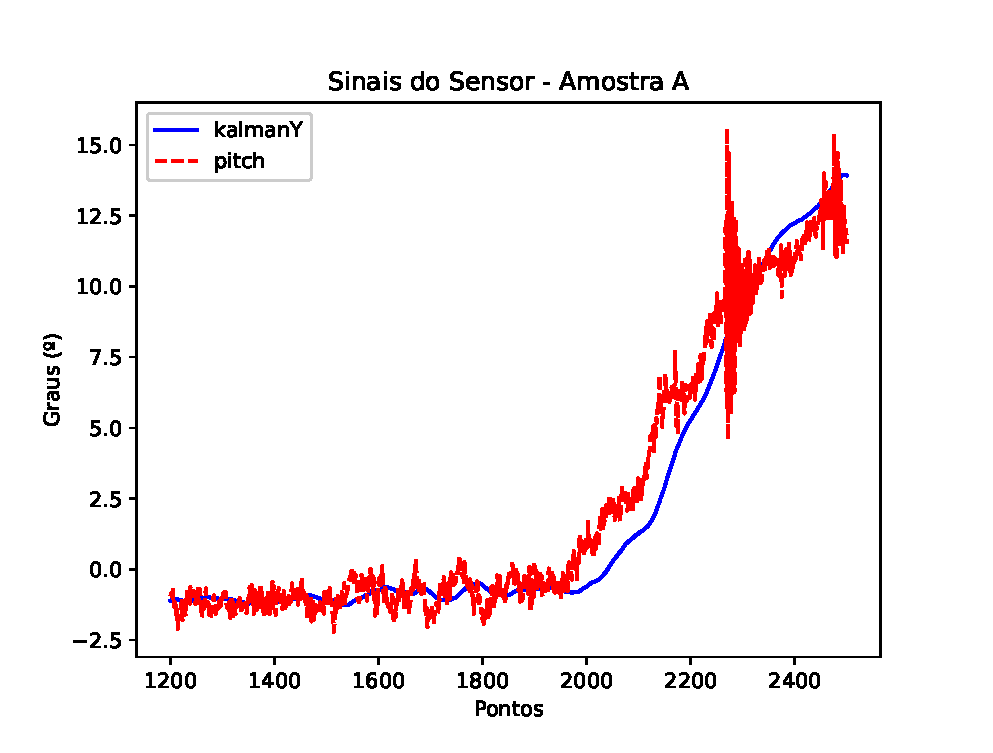
\includegraphics[width=8cm]{Resultados/sinaisAmostraA.eps}
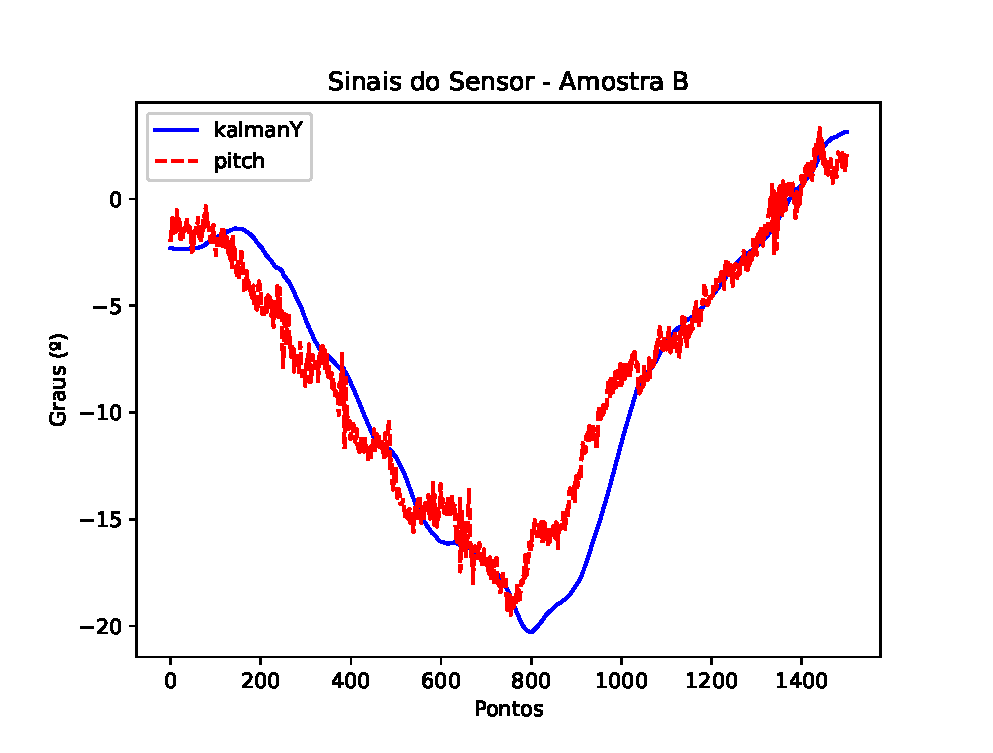
\includegraphics[width=8cm]{Resultados/sinaisAmostraB.eps}
\caption{Comportamento de forma macro do sinal do sensor filtrado, curva azul e do sinal real, curva vermelha.}
\label{fig:sinaisMacroSensor} 
\end{figure}

Para uma melhor visualização da curva, plotou-se apenas uma pequena fatia dos dados da amostra B, como mostra a Figura (\ref{fig:sinaisFatiadoSensor}). Aqui, verifica-se e comprova o que foi dito, que a sensibilidade a ruído do sinal real é bem alta e que o sinal filtrado segue a curva real de forma bem suave.

\begin{figure}[H]
\centering
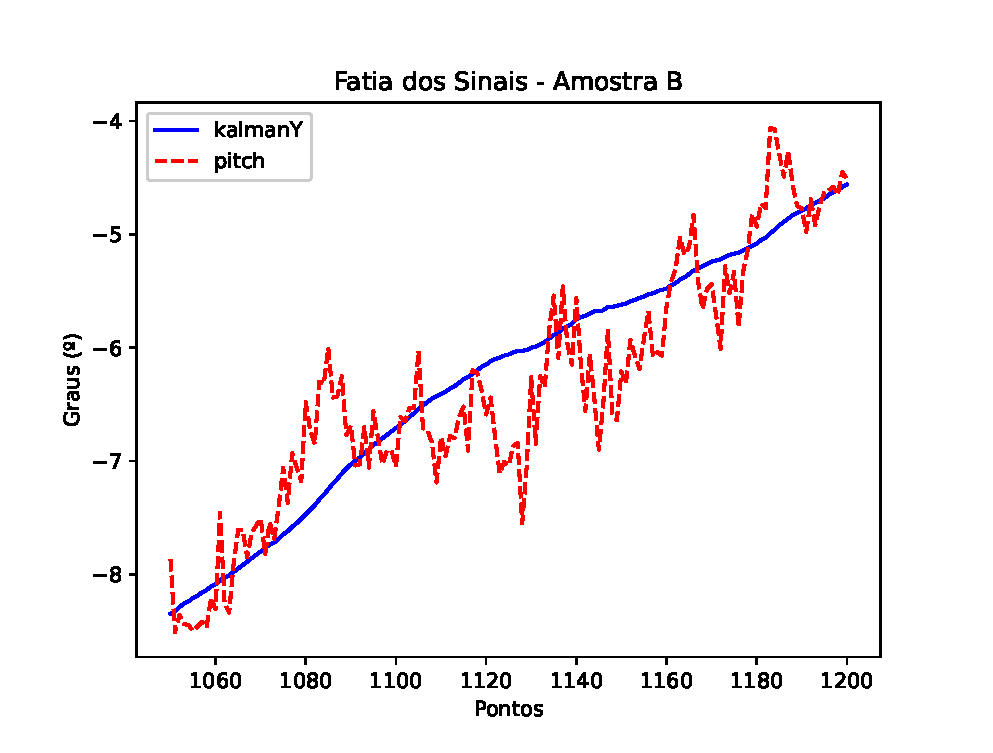
\includegraphics[scale=0.75]{Resultados/fatiaSinalSensor.eps}
\caption{Comportamento de forma micro dos dois sinais do sensor.}
\label{fig:sinaisFatiadoSensor} 
\end{figure}

\subsection{Validação dos Motores}

\section{Aplicação do Controlador}


\chapter{Considerações Finais}

Neste capítulo são apresentadas as considerações decorrentes dos resultados obtidos no desenvolvimento deste trabalho e a proposta de continuidade para o estudo.

\section{Conclusões}

O objetivo deste trabalho foi desenvolver uma planta física de controle como parte da disciplina de trabalho de conclusão de curso, utilizando técnica de controle ótimo para sistema não linear. Além disso, utilizou-se de vários outros conceitos abordados ao longo do curso, tais como desenho e cálculos mecânicos, eletrônica e circuitos elétricos e programação para computadores.

Com relação ao tema abordado, conclui-se que é de grande importância na academia e que possui uma variedade de pesquisas já realizadas em relação a este sistema. A técnica de modelagem utilizada é bastante usual na literatura.

Em relação as técnicas de controle ótimo, há vários estudos sobre, o que assegurou uma maior certeza na escolha do controlador implementado. O projeto do controlador LQG por meio de ajuda de \textit{software}, como o MATLAB, mostrou ser fácil de se implementar em simulação e na prática. Em simulação, os resultados obtidos com relação ao sistema não linear, foi bastante eficaz mesmo lidando com distúrbios e ruídos aplicados.

Ao fim da montagem da estrutura mecânica e do circuito eletrônico, realizou-se a validação do sensor e dos motores. Observou-se a sensibilidade para ruído do do sinal real vindo do sensor e a robustez do sinal filtrado. Em relação aos motores, obteve-se os máximos e mínimos de PWM e sentido de giro de cada motor.
Ao aplicar o controlador, notou-se a diferença de velocidade em cada roda, fazendo a estrutura girar. Esse acontecimento era esperado uma vez que não há controle dos motores, apenas da posição angular da estrutura. O intuito ao aplicar o LQG era o controle na vertical da estrutura....

Com o presente trabalho foi possível desenvolver habilidades extras da área de controle que não são abordadas na grade curricular do curso. A experiência adquirida nas disciplinas teóricas bem como as de laboratórios foram de
suma importância para atingir os resultados alcançados. Contudo, como já citado, este trabalho é multidisciplinar e que necessitou de utilizar de vários fundamentos adquiridos ao longo do curso.


\section{Propostas de Trabalhos Futuros}

A partir da experiência adquirida durante o desenvolvimento deste trabalho, foram elencados os seguintes tópicos como possíveis continuações do estudo:

\begin{itemize}
    \item Identificação de parâmetros aqui descartados, afim de simplificar o modelo, como a fricção e averiguar a necessidade de adição;
    \item Identificação mais robusta dos parâmetros mecânicos e elétricos dos motores utilizados;
    \item Implementação do uso dos \textit{encoders} dos motores, o que acarretaria em uma adição de dois novos estados na modelagem, posição e velocidade linear;
    \item Um outra abordagem é da utilização de motores de passo ao invés de motores de corrente contínua, uma vez que os motores passo tem um ótimo controle de posição e são muito precisos.
    \item Implementação de novas técnicas de controle para efeito de comparação com a abordada neste trabalho;
    \item Utilização de técnicas de controle MIMO (múltiplas entradas e múltiplas saídas), como a realização de um controlador em cascata para o controle da posição linear e da vertical.

\end{itemize}

% Apêndices
%\appendix
    %\chapter{Códigos}\label{Apendice:CodigoMatlab}
%\pagenumbering{arabic}

\begin{minted}[breaklines=true]{C}

Link para códigos e modelagem completa do trabalho: https://github.com/mferreiracosta/tcc_cefet

%% PROGRAMA PÊNDULO INVERTIDO - TCC 2 - 2022.1
% Autor: Matheus Ferreira Costa
% Orientador: Luís Filipe 

clc; clear all; close all

%% Definição dos Parâmetros
syms g M m L r R kt

g = 9.80665;
M = 0.066;    
m = 0.788;
L = 0.18;    r = 0.033;
R = 0.92;    kt = 0.54;

den = 2*M*r^2 + m*(r^2 + L^2 + 2*L*r);

%% Calculando as matrizes do sistema A, B, C e D

A = [      0      1;
     (m*g*L)/den  0];
B = [0; kt/(R*den)];
C = [1 0];
D = [0];

sys = ss(A,B,C,D);

%% Calculando o rank de controlabilidade e observabilidade do sistema
Sc = ctrb(sys);
So = obsv(sys);

rank_ctrb = rank(Sc);
rank_obsv = rank(So);

%% Escolhendo as matrizes Q e R para calcular o controlador LQR
Q = [1   0;            
     0   1];
R = 1;

%% Construção do Sistema em Espaço de Estados no Tempo Discreto
Ts = 0.05;
sysd = c2d(sys,Ts);

% Matrizes discretas: Ad e Bd, Cd = C e Dd = D
Ad = sysd.a;
Bd = sysd.b;

%% Construção do controlador LQR no Tempo Discreto
[Krd,S,e] = dlqr(Ad,Bd,Q,R);

%% Construção do LQE - Filtro de Kalman no Tempo Discreto
Qo = 1;                  % matriz de covariância do distúrbio           
Ro = 1;                  % (escalar) covariância do ruído de medição  

% Construção do LQE - Filtro de Kalman
[kalmf,Lkalm,P] = kalman(sysd,Qo,Ro);

Ld = dlqr(Ad',C',Qo,Ro);
Ld = Ld';

sysKFd = ss(Ad-Ld*C,[Bd Ld],eye(2),zeros(2,2));

\end{minted}
    %\chapter{Complemento}
%\pagenumbering{arabic}

Você não acha que para um TCC vc está colocando apêndices demais? O
relatório não deve ter {\em tudo} que vc estudou ou fez, mas um trabalho
com início meio e fim!

Uma referência utilizada neste trabalho foi produzida por
Michigan University \citeyearpar{MU:14}.

%========= Referências ====================
\cleardoublepage
\phantomsection
\addcontentsline{toc}{chapter}{Referências}
\renewcommand{\bibname}{Referências}
\markboth{Referências}{Referências}

% Define o estilo da citação e da bibliografia
\bibliographystyle{abnt}
% Define os arquivos onde estão cadastradas as referências bibliográficas
\bibliography{meubib}

\end{document}
